\documentclass[10pt]{beamer}
\usetheme{Warsaw}
\usecolortheme{beaver}

\usepackage{amssymb, amsmath, amsfonts}
\usepackage{moreverb}
\usepackage{graphicx}
\usepackage{enumerate}
\usepackage{graphics}
\usepackage{color}
\usepackage{array}
\usepackage{float}
\usepackage{hyperref}
\usepackage{textcomp}
\usepackage{alltt}
\usepackage{mathtools}
\usepackage{tikz}
\usetikzlibrary{positioning}
\usetikzlibrary{arrows}
\usepackage{pgfplots}
\usepackage{bigints}

\newcommand{\suchthat}{\, \mid \,}
\renewcommand{\theenumi}{\alph{enumi}}
\newcommand\Wider[2][3em]{%
\makebox[\linewidth][c]{%
  \begin{minipage}{\dimexpr\textwidth+#1\relax}
  \raggedright#2
  \end{minipage}%
  }%
}

\pgfmathdeclarefunction{gauss}{2}{%
  \pgfmathparse{1/(#2*sqrt(2*pi))*exp(-((x-#1)^2)/(2*#2^2))}%
}

\setcounter{section}{-1}
%\setlength{\jot}{30pt}

\title{The Effects of Intraspecific Genetic Variation on the Dynamics of Predator-Prey Ecological Communities}
\author{\vspace{-15pt} Sam Fleischer, Pablo Chavarria}
\date{\vspace{-5pt} May 3, 2015}

\begin{document}

\begin{frame}
	\titlepage
	\begin{center}
		{\bf Preparing Undergraduates through Mentoring for PhDs (PUMP) Research Symposium}
	\end{center}
	\begin{align*}
		\begin{array}{lll}
		\text{Advisor:} & \text{Dr. Jing Li, Mathematics,} & \text{CSU Northridge} \\
		\text{Consultant:} & \text{Dr. Casey terHorst, Biology,} & \text{CSU Northridge} \\
		\text{Supported By:} & \text{Pacific Math Alliance, PUMP,} & \text{CSU Northridge}
		\end{array}
	\end{align*}
\end{frame}

\begin{frame}
	\frametitle{Overview}
	\begin{itemize}
		\item Motivation
		\begin{itemize}
			\item Observations in Nature
			\item Previous Models
		\end{itemize}
		\item Our Expansions
		\begin{itemize}
			\item Gaussian Attack Rate under Coevolution
			\item Introduce Stabilizing Selection
			\item General Ditrophic Expansion
		\end{itemize}
		\item Discussion
	\end{itemize}
\end{frame}

\section{Motivation}
\subsection{Observations in Nature}
\begin{frame}
	\frametitle{Observations in Nature}
	\begin{minipage}{0.65\textwidth}
		\begin{itemize}
			\item Predator/Prey interactions are prevalent in nature
			\begin{itemize}
				\item Crab vs. gastropod {\tiny[Saloniemi, 1993]}
				\item Classical Lotka-Volterra model
				\begin{itemize}
					\item Genetic adaptation is insignificant
				\end{itemize}
			\end{itemize} \vspace{15pt}
			\uncover<2->{\item There is trait variation within species, which causes {\bf variation in fundametal model parameters}
			\begin{itemize}
				% \item Thickness of plant cuticula {\tiny[Saloniemi, 1993]}
				\item Relative strength of crab claw vs. gastropod shell {\tiny[Saloniemi, 1993]}
				\item Incorporating trait variation provides {\bf richer dynamics} than classical Lotka-Volterra models
			\end{itemize}}
		\end{itemize}
	\end{minipage}
	\begin{minipage}{0.25\textwidth}
		\begin{figure}
			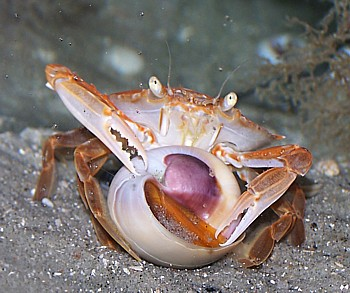
\includegraphics[width=1.5\textwidth]{figures/crab_eating_gastropod.jpg}
		\end{figure}
	\end{minipage}
\end{frame}

\subsection{Previous Models}
\begin{frame}
	\frametitle{Classical Lotka-Volterra Model}
	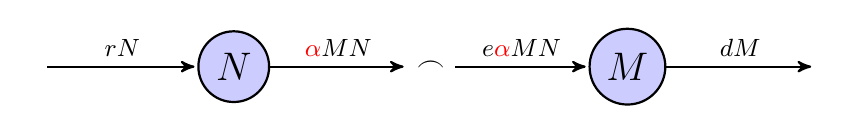
\begin{tikzpicture}[->,>=stealth',shorten >=1pt,auto,node distance=2.5cm, thick,main node/.style={circle,fill=blue!20,draw,font=\sffamily\Large\bfseries}]

		\node[main node] (1) {$N$};
		\node (midpt) [right of=1] {$\frown$};
		\node[main node] (2) [right of=midpt] {$M$};
		\node (input) [left of=1] {};
		\node (output) [right of=2] {};

		\path[every node/.style={font=\sffamily\small}]
		(input)	edge node {$rN$} (1)
		(1)		edge node {${\color{red}\alpha} MN$} (midpt)
		(midpt)	edge node {$e{\color{red}\alpha} MN$} (2)
		(2)		edge node {$dM$} (output);
	\end{tikzpicture}\vskip0.75cm
	\begin{columns}
    		\begin{column}{0.4\textwidth}
			\begin{align*}
				\frac{dN}{dt} &= N(r - {\color{red}\alpha} M)\\[.1cm]
				\frac{dM}{dt} &= M(e{\color{red}\alpha} N - d)
			\end{align*}
    		\begin{itemize}
    			\item \footnotesize Prey Exponential Growth
    			\item Predator Exponential Decay
    			\item Linear Functional Response
    		\end{itemize}
   		 \end{column}
		 \begin{column}{0.60\textwidth}
			{\bf Variables}
			\begin{itemize}
				\item $N \equiv $ Prey Density
				\item $M \equiv $ Predator Density
			\end{itemize}
			{\bf Parameters}
			\begin{itemize}
				\item {\color{red}$\alpha \equiv $ Attack rate\uncover<2->{\ \ \ \ \ $\longleftarrow$ {\bf No variation!}}}
				\item $r \equiv $ Prey Growth rate
				\item $e \equiv $ Efficiency
				\item $d \equiv $ Predator death rate
			\end{itemize}
		\end{column}
	\end{columns}
\end{frame}
\begin{frame}
	\frametitle{Schreiber, B\"urger, and Bolnick's Expansion}
	{\bf Assume the {\color{red}Predator Species} has a normally distributed trait value.}
	\begin{align*}
		p({\color{red}m}, \overline{m}) &= \frac{1}{\sqrt{2\pi\sigma^2}}\exp\left[{-\frac{({\color{red}m} - \overline{m})^2}{2\sigma^2}}\right]
	\end{align*}
	\uncover<2->{{\bf Attack Rate is a Function of the {\color{red}Predator's Trait Value}}
	\begin{align*}
		a({\color{red}m}) &= \alpha \exp\left[-\frac{({\color{red}m} - {\color{cyan}\theta})^2}{2\tau^2}\right]
	\end{align*}}
	\begin{columns}
		\begin{column}{0.45\textwidth}
			{\bf Variables}
			\begin{itemize}
				\item {\color{red}$m \equiv $ Predator Trait Value}
				\item \uncover<3->{{\color{blue} (((No Prey Trait Value)))}}
			\end{itemize}
		\end{column}
		\begin{column}{0.60\textwidth}
			{\bf Parameters}
			\begin{itemize}
				\item $\sigma^2 \equiv $ Predator Trait Variance
				\item \uncover<2->{$\alpha \equiv $ Maximum attack rate}
				\item \uncover<2->{$\tau \equiv $ Specialization Constant}
				\item \uncover<2->{{\color{cyan}$\theta \equiv $ Optimal trait value \uncover<3->{\\ \ \ \ \ \ \ $\uparrow$ {\bf No variation!}}}}
			\end{itemize}
		\end{column}
	\end{columns}
\end{frame}

\section{Our Expansions}
\subsection{Coevolution Model}
\begin{frame}
	\frametitle{Normally Distributed Trait Values}
	{\bf Assume {\color{blue}Prey} and {\color{red}Predator} have normally distributed trait values.}
	\begin{align*}
		p({\color{blue}n}, {\color{blue}\overline{n}}) &= \frac{1}{\sqrt{2\pi\beta^2}}\exp\left[{-\frac{({\color{blue}n} - {\color{blue}\overline{n}})^2}{2\beta^2}}\right]
	\end{align*}
	\begin{align*}
		p({\color{red}m}, {\color{red}\overline{m}}) &= \frac{1}{\sqrt{2\pi\sigma^2}}\exp\left[{-\frac{({\color{red}m} - {\color{red}\overline{m}})^2}{2\sigma^2}}\right]
	\end{align*}
	\begin{columns}
		\begin{column}{0.50\textwidth}
			{\bf Variables}
			\begin{itemize}
				\item \footnotesize{\color{blue}$n \equiv $ Prey Trait Value}
				\item {\color{blue}$\overline{n} \equiv $ {\bf Average} Prey Trait Value}
				\item {\color{red}$m \equiv $ Predator Trait Value}
				\item {\color{red}$\overline{m} \equiv $ {\bf Average} Predator Trait Value}
			\end{itemize}
		\end{column}
		\begin{column}{0.42\textwidth}
			{\bf Parameters}
			\begin{itemize}
				\item \footnotesize$\beta^2 \equiv $ Prey Trait Variance
				\item $\sigma^2 \equiv $ Predator Trait Variance
			\end{itemize}
		\end{column}
	\end{columns}
\end{frame}

\begin{frame}
	\vspace{-5pt}
	\frametitle{Attack Rate}
	{\bf Attack Rate is a Gaussian Function of the {\color{blue}Prey's Trait Value} and the {\color{red}Predator's Trait Value}}
	\vspace{-7pt}
	\begin{align*}
		a({\color{blue}n}, {\color{red}m}) &= \alpha \exp\left[-\frac{(({\color{red}m} - {\color{blue}n}) - {\color{cyan}\theta})^2}{2\tau^2}\right]
	\end{align*}
	\uncover<2->{\vspace{-7pt}
	{\bf Average Attack Rate}
	\begin{align*}
		\overline{a}({\color{blue}\overline{n}}, {\color{red}\overline{m}}) &= \int_{-\infty}^{\infty}\int_{\-\infty}^{\infty} a({\color{blue}n}, {\color{red}m}) \cdot p({\color{blue}n}, {\color{blue}\overline{n}}) \cdot p({\color{red}m}, {\color{red}\overline{m}})\ d{\color{blue}n} d{\color{red}m} \\
		&= \frac{\alpha\tau}{\sqrt{\sigma^2 + \beta^2 + \tau^2}}\exp\left[{-\frac{(({\color{red}\overline{m}} - {\color{blue}\overline{n}}) - {\color{cyan}\theta})^2}{2(\sigma^2 + \beta^2 + \tau^2)}}\right]
	\end{align*}}
	\vspace{-5pt}
	\begin{columns}
		\begin{column}{0.50\textwidth}
			{\bf Variables}
			\begin{itemize}
				\item \footnotesize{\color{blue}$n \equiv $ Prey Trait Value}
				\item {\color{blue}$\overline{n} \equiv $ {\bf Average} Prey Trait Value}
				\item {\color{red}$m \equiv $ Predator Trait Value}
				\item {\color{red}$\overline{m} \equiv $ {\bf Average} Predator Trait Value}
			\end{itemize}
		\end{column}
		\begin{column}{0.42\textwidth}
			{\bf Parameters}
			\begin{itemize}
				\item \footnotesize$\alpha \equiv $ Maximum attack rate
				\item {\color{cyan}$\theta \equiv $ Optimal trait \bf difference}
				\item $\tau^2 \equiv $ Specialization Constant
				\item \uncover<2->{$\beta^2 \equiv $ Prey Trait Variance}
				\item \uncover<2->{$\sigma^2 \equiv $ Predator Trait Variance}
			\end{itemize}
		\end{column}
	\end{columns}
\end{frame}
\begin{frame}
	\frametitle{Fitness Assumptions}
	\begin{itemize}
		\item Prey experiences {\color{blue}logistic growth} in absence of predator
		\item Predator experiences {\color{red}exponential decay} in absence of prey
	\end{itemize}
	\begin{align*}
		Y(N, n, M, m) &= {\color{blue}r\left(1 - \frac{N}{K}\right)} - Ma(n, m) \\[.1cm]
		W(N, n, M, m) &= eNa(n, m)\ {\color{red}-\ d}
	\end{align*}
	\begin{columns}
		\begin{column}{0.45\textwidth}
			{\bf Variables}
			\begin{itemize}
				\item \footnotesize$N \equiv $ Prey Density
				\item $n \equiv $ Prey Trait Value
				\item $M \equiv $ Predator Density
				\item $m \equiv $ Predator Trait Value
			\end{itemize}
		\end{column}
		\begin{column}{0.55\textwidth}
			{\bf Parameters}
			\begin{itemize}
				\item \footnotesize{\color{blue}$r \equiv $ Intrinsic Prey Growth Rate}
				\item {\color{blue}$K \equiv $ Prey Carrying Capacity}
				\item {\color{red}$d \equiv $ Predator Death Rate}
				\item $e \equiv $ Efficiency
			\end{itemize}
		\end{column}
	\end{columns}
\end{frame}
\begin{frame}
	\frametitle{Average Fitness}
	\begin{align*}
	{\color{blue}\overline{Y}(N, \overline{n}, M, \overline{m})} &= \int_{-\infty}^{\infty}\int_{-\infty}^{\infty} Y(N, n, M, m) \cdot p(m, \overline{m}) \cdot p(n, \overline{n})\ dm dn \\
	&= {\color{blue}r\left(1 - \frac{N}{K}\right) - M\overline{a}(\overline{n}, \overline{m})} \\[.1cm]
	{\color{red}\overline{W}(N, \overline{n}, M, \overline{m})} &= \int_{-\infty}^{\infty}\int_{-\infty}^{\infty} W(N, n, M, m) \cdot p(m, \overline{m}) \cdot p(n, \overline{n})\ dm dn \\
	&= {\color{red}eN\overline{a}(\overline{n}, \overline{m}) - d}
	\end{align*}
	\begin{columns}
		\begin{column}{0.5\textwidth}
			{\bf Variables}
			\begin{itemize}
				\item \footnotesize{\color{blue}$N \equiv $ Prey Density}
				\item {\color{blue}$\overline{n} \equiv $ {\bf Average} Prey Trait Value}
				\item {\color{red}$M \equiv $ Predator Density}
				\item {\color{red}$\overline{m} \equiv $ {\bf Average} Predator Trait Value}
			\end{itemize}
		\end{column}
		\begin{column}{0.5\textwidth}
			{\bf Parameters}
			\begin{itemize}
				\item \footnotesize$r \equiv $ Intrinsic Prey Growth Rate
				\item $K \equiv $ Prey Carrying Capacity
				\item $d \equiv $ Predator Death Rate
				\item $e \equiv $ Efficiency
			\end{itemize}
		\end{column}
	\end{columns}
\end{frame}
\begin{frame}
	\frametitle{Ecological Components}
	\vspace{-10pt}
	\begin{align*}
		\frac{dN}{dt} &= N\cdot {\color{blue}\overline{Y}(N, \overline{n}, M, \overline{m})}\ = N{\color{blue}\left[r\left(1 - \frac{N}{K}\right) - M\overline{a}(\overline{n}, \overline{m})\right]}\\[.1cm]
		\frac{dM}{dt} &= M\cdot {\color{red}\overline{W}(N, \overline{n}, M, \overline{m})} = M{\color{red}\left[eN\overline{a}(\overline{n}, \overline{m}) - d\right]}
	\end{align*}
	\begin{center}
		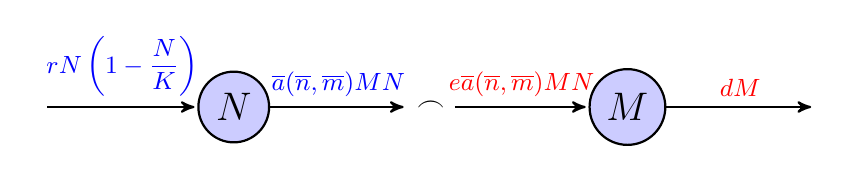
\begin{tikzpicture}[->,>=stealth',shorten >=1pt,auto,node distance=2.5cm, thick,main node/.style={circle,fill=blue!20,draw,font=\sffamily\Large\bfseries}]
	
			\node[main node] (1) {$N$};
			\node (midpt) [right of=1] {$\frown$};
			\node[main node] (2) [right of=midpt] {$M$};
			\node (input) [left of=1] {};
			\node (output) [right of=2] {};
	
			\path[every node/.style={font=\sffamily\small}]
			(input)	edge node {{\color{blue}$rN\left(1 - \dfrac{N}{K}\right)$}} (1)
			(1)		edge node {{\color{blue}$\overline{a}(\overline{n}, \overline{m})MN$}} (midpt)
			(midpt)	edge node {{\color{red}$e\overline{a}(\overline{n}, \overline{m})MN$}} (2)
			(2)		edge node {{\color{red}$dM$}} (output);
		\end{tikzpicture}\vskip0.35cm
	\end{center}
	\begin{columns}
		\begin{column}{0.5\textwidth}
			{\bf Variables}
			\begin{itemize}
				\item \footnotesize{\color{blue}$N \equiv $ Prey Density}
				\item {\color{blue}$\overline{n} \equiv $ {\bf Average} Prey Trait Value}
				\item {\color{red}$M \equiv $ Predator Density}
				\item {\color{red}$\overline{m} \equiv $ {\bf Average} Predator Trait Value}
			\end{itemize}
		\end{column}
		\begin{column}{0.5\textwidth}
			{\bf Parameters}
			\begin{itemize}
				\item \footnotesize$r \equiv $ Intrinsic Prey Growth Rate
				\item $K \equiv $ Prey Carrying Capacity
				\item $d \equiv $ Predator Death Rate
				\item $e \equiv $ Efficiency
			\end{itemize}
		\end{column}
	\end{columns}
\end{frame}
\begin{frame}
	\frametitle{Evolutionary Components}
	\begin{itemize}
		\item The evolution of the mean trait value is always \underline{in the direction} \underline{which increases the mean fitness in the population}. {\tiny[Lande, 1976]}
	\end{itemize}
	\begin{align*}
		\frac{d\overline{n}}{dt} &= \beta_G^2{\color{cyan}\frac{\partial \overline{Y}}{\partial \overline{n}}} = \beta_G^2{\color{cyan}\frac{M(\theta - (\overline{m} - \overline{n}))}{\sigma^2 + \beta^2 + \tau^2} \overline{a}(\overline{n}, \overline{m})}\\[.1cm]
		\frac{d\overline{m}}{dt} &= \sigma_G^2{\color{magenta}\frac{\partial \overline{W}}{\partial \overline{m}}} = \sigma_G^2{\color{magenta}\frac{eN(\theta - (\overline{m} - \overline{n}))}{\sigma^2 + \beta^2 + \tau^2} \overline{a}(\overline{n}, \overline{m})}
	\end{align*}
	\vskip.25cm
	\begin{columns}
		\begin{column}{0.5\textwidth}
			{\bf Variables}
			\begin{itemize}
				\item \footnotesize$N \equiv $ Prey Density
				\item $\overline{n} \equiv $ Mean Prey Character
				\item $M \equiv $ Predator Density
				\item $\overline{m} \equiv $ Mean Predator Character
			\end{itemize}
		\end{column}
		\begin{column}{0.5\textwidth}
			{\bf Parameters}
			\begin{itemize}
				\item \footnotesize$\beta_G^2 \equiv $ Prey genetic variance
				\item $\sigma_G^2 \equiv $ Predator genetic variance
			\end{itemize}
		\end{column}
	\end{columns}
\end{frame}
\begin{frame}
	\frametitle{The Complete $1\times1$ Model \\ (One Prey Species, One Predator Species)}
	{\bf Ecological Components}
	\begin{align*}
		\frac{dN}{dt} &= N\cdot {\color{blue}\overline{Y}(N, \overline{n}, M, \overline{m})}\ \ =\ N{\color{blue}\left[r\left(1 - \frac{N}{K}\right) - M\overline{a}(\overline{m}, \overline{n})\right]}\\[.1cm]
		\frac{dM}{dt} &= M\cdot {\color{red}\overline{W}(N, \overline{n}, M, \overline{m})}\ \ \ \ \ =\ M{\color{red}\left[eN\overline{a}(\overline{m}, \overline{n}) - d\right]}
	\end{align*}
	{\bf Evolutionary Components}
	\begin{align*}
		\frac{d\overline{n}}{dt} &= \beta_G^2{\color{cyan}\frac{\partial \overline{Y}}{\partial \overline{n}}} = \beta_G^2{\color{cyan}\frac{M(\theta - (\overline{m} - \overline{n}))}{\sigma^2 + \beta^2 + \tau^2} \overline{a}(\overline{n}, \overline{m})}\\[.1cm]
		\frac{d\overline{m}}{dt} &= \sigma_G^2{\color{magenta}\frac{\partial \overline{W}}{\partial \overline{m}}} = \sigma_G^2{\color{magenta}\frac{eN(\theta - (\overline{m} - \overline{n}))}{\sigma^2 + \beta^2 + \tau^2} \overline{a}(\overline{n}, \overline{m})}
	\end{align*}
\end{frame}

\begin{frame}
	\frametitle{Equilibria - $1\times1$}
	{\bf Extinction} \uncover<2->{$\boxed{\text{\it Unstable}}$}
	\begin{align*}
		({\color{blue}N^*}, {\color{red}M^*}, {\color{cyan}\overline{n}^*}, {\color{magenta}\overline{m}^*}) = ({\color{blue}0}, {\color{red}0}, {\color{cyan}\underline{\ \ }}, {\color{magenta}\underline{\ \ }})
	\end{align*}
	\uncover<3->{{\bf Exclusion}
	\begin{align*}
		({\color{blue}N^*}, {\color{red}M^*}, {\color{cyan}\overline{n}^*}, {\color{magenta}\overline{m}^*}) = ({\color{blue}K}, {\color{red}0}, {\color{cyan}\mu^*}, {\color{magenta}\mu^* + \theta})\ \ \ \ \ \ \ \ \ \ \ \ \ \ \ \ \ \text{where $\mu^*$ is arbitrary}
	\end{align*}}
	\uncover<4->{
		{\it Necessary Condition for Asymptotically $\boxed{Stable}$ Exclusion:}
		\begin{align*}
			d > \dfrac{Ke\alpha\tau}{\sqrt{A}} \hphantom{mmmmmmmmm} \text{where A = $\sigma^2 + \beta^2 + \tau^2$}
		\end{align*}}
\end{frame}
\begin{frame}
	\frametitle{Equilibria - $1\times1$}
	{\bf Coexistence}
	\begin{align*}
		({\color{blue}N^*}, {\color{red}M^*}, {\color{cyan}\overline{n}^*}, {\color{magenta}\overline{m}^*}) = ({\color{blue}\dfrac{d\sqrt{A}}{e \alpha \tau}}\ ,\ {\color{red}\dfrac{r\sqrt{A}}{\alpha\tau}\left(1 - \dfrac{d\sqrt{A}}{Ke\alpha\tau}\right)}\ ,\ {\color{cyan}\mu^*}\ ,\ {\color{magenta}\mu^* + \theta})
		\end{align*}
	\uncover<2->{
		{\it Necessary Condition for Asymptotically $\boxed{Stable}$ Coexistence:}
		\begin{align*}
			\dfrac{\sigma_G^2}{\beta_G^2} > \dfrac{r}{d}\left(1 - \dfrac{d\sqrt{A}}{Ke\alpha\tau}\right)
		\end{align*}}
\end{frame}

\begin{frame}
	\frametitle{Figures - $1\times1$ - Stable Exclusion}
	\Wider[6em]{
	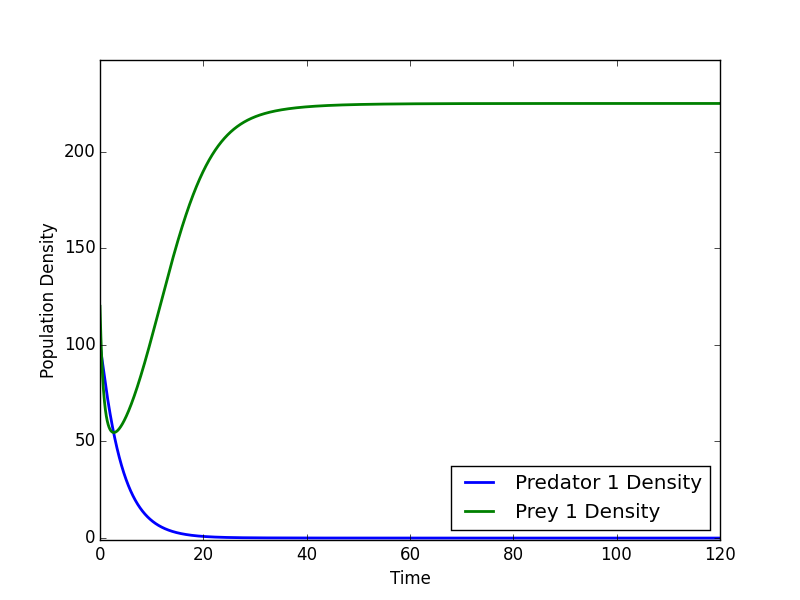
\includegraphics[scale=0.3175]{figures/1x1/constant_growth/densities_exclusion.png}
   	\hfill
   	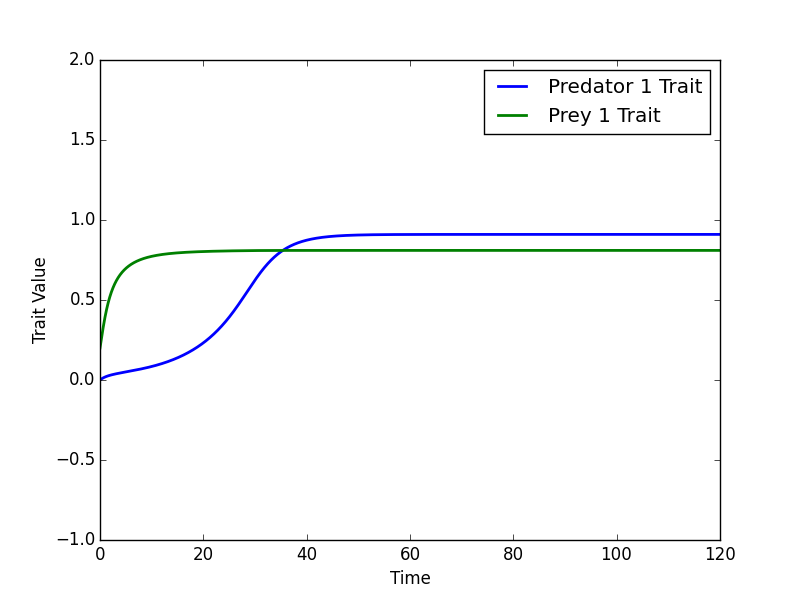
\includegraphics[scale=0.3175]{figures/1x1/constant_growth/traits_exclusion.png}
	}
\end{frame}
\begin{frame}
	\frametitle{Figures - $1\times1$ - Stable Coexistence}
	\Wider[6em]{
	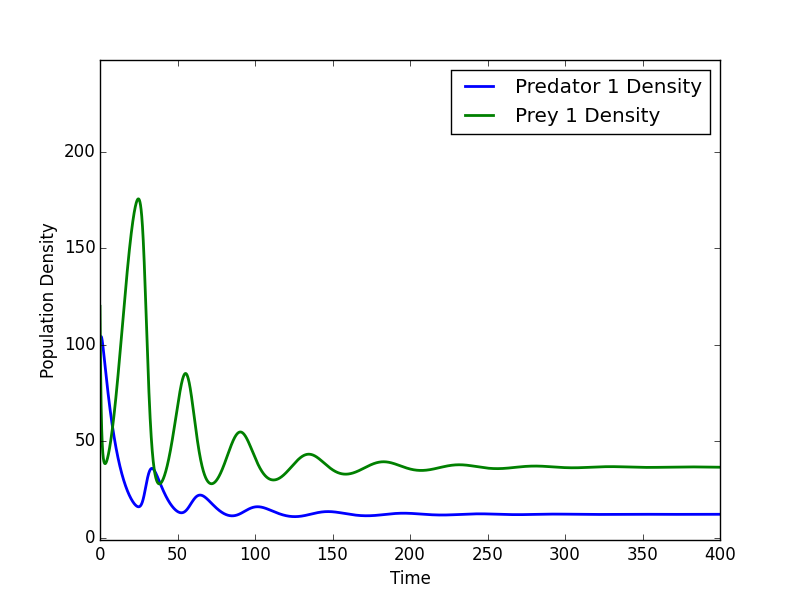
\includegraphics[scale=0.3175]{figures/1x1/constant_growth/densities_stable_coexistence.png}
   	\hfill
   	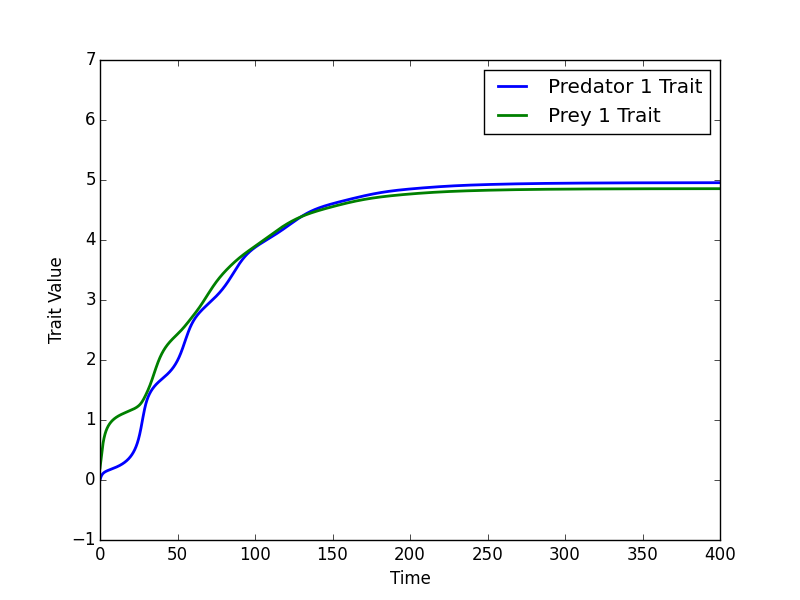
\includegraphics[scale=0.3175]{figures/1x1/constant_growth/traits_stable_coexistence.png}
	}
\end{frame}
\begin{frame}
	\frametitle{Figures - $1\times1$ - ``Arms Race'' Coexistence}
	\Wider[6em]{
	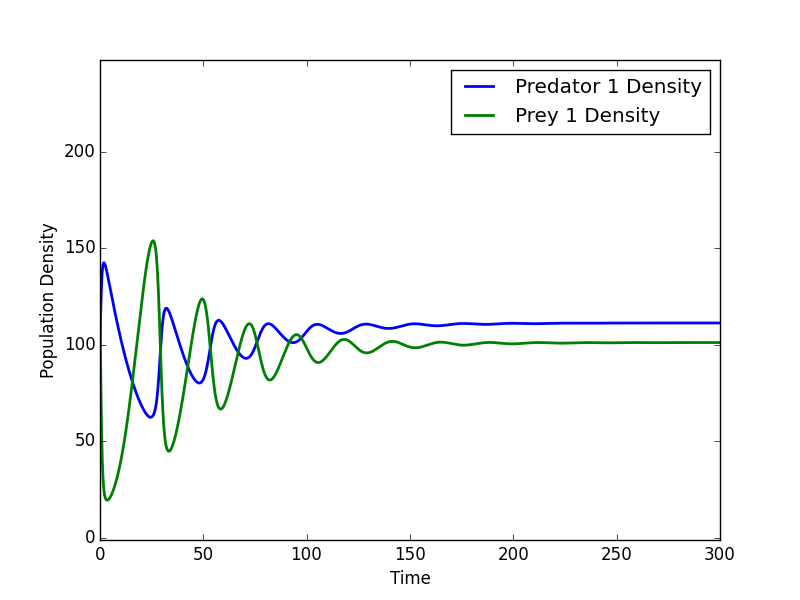
\includegraphics[scale=0.3175]{figures/1x1/constant_growth/densities_unstable_coexistence.png}
   	\hfill
   	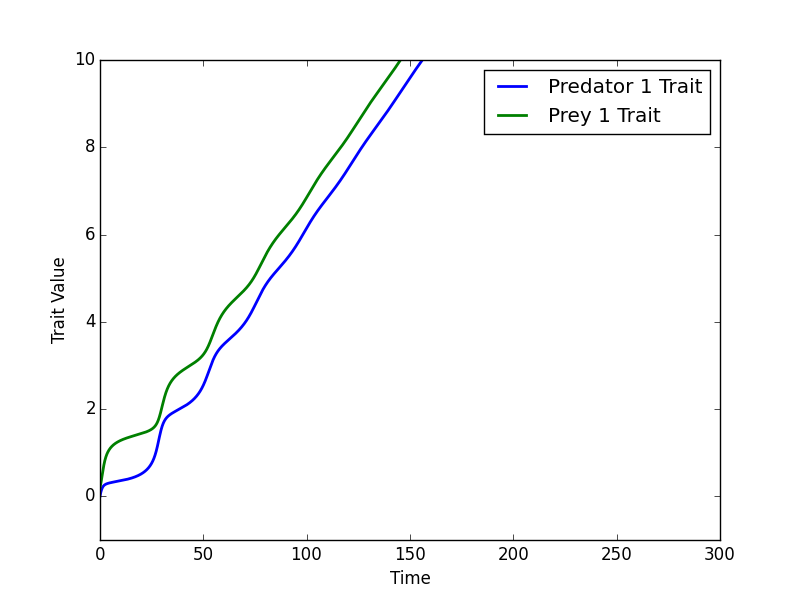
\includegraphics[scale=0.3175]{figures/1x1/constant_growth/traits_unstable_coexistence.png}
	}
\end{frame}

\subsection{Stabilizing Selection}
\begin{frame}
	\frametitle{Avoiding an ``Arms Race'' with Stabilizing Selection}
	{\bf Assume Prey Growth Rate is a Function of the {\color{blue}Prey's Trait Value}}
	\begin{align*}
		r({\color{blue}n}) &= \rho \exp\left[-\frac{({\color{blue}n} - {\color{cyan}\phi})^2}{2\gamma^2}\right]
	\end{align*}
	\uncover<2->{{\bf Averge Growth Rate}}
	\uncover<2->{\begin{align*}
		\overline{r}({\color{blue}\overline{n}}) &= \int_{-\infty}^{\infty}r({\color{blue}n}) \cdot p({\color{blue}n}, {\color{blue}\overline{n}}) d{\color{blue}n} \\
		&= \frac{\rho\gamma}{\sqrt{\beta^2 + \gamma^2}}\exp{\left[-\frac{({\color{blue}n} - {\color{cyan}\phi})^2}{2\gamma^2}\right]}
	\end{align*}}
	\begin{columns}
		\begin{column}{0.42\textwidth}
			{\bf Variables}
			\begin{itemize}
				\item \footnotesize{\color{blue}$n \equiv $ Prey Trait Value}
				\item {\color{blue}$\overline{n} \equiv $ {\bf Average} Prey Trait Value}
			\end{itemize}
		\end{column}
		\begin{column}{0.48\textwidth}
			{\bf Parameters}
			\begin{itemize}
				\item \footnotesize$\rho \equiv $ Maximum Growth Rate
				\item {\color{cyan}$\phi \equiv $ Prey Optimum Trait Value}
				\item $\gamma^2 \equiv $ Stabilizing Selection Constant
				\item \uncover<2->{$\beta^2 \equiv $ Prey Trait Variance}
			\end{itemize}
		\end{column}
	\end{columns}
\end{frame}
\begin{frame}
	\frametitle{Fitness Assumptions}
	\begin{itemize}
		\item Prey experiences {\color{blue}logistic growth} in absence of predator
		\item Predator experiences {\color{red}exponential decay} in absence of prey
	\end{itemize}
	\begin{align*}
		Y(N, n, M, m) &= {\color{blue}r(n)\left(1 - \frac{N}{K}\right)} - Ma(n, m) \\[.1cm]
		W(N, n, M, m) &= eNa(n, m)\ {\color{red}-\ d}
	\end{align*}
	\begin{columns}
		\begin{column}{0.45\textwidth}
			{\bf Variables}
			\begin{itemize}
				\item \footnotesize$N \equiv $ Prey Density
				\item $n \equiv $ Prey Trait Value
				\item $M \equiv $ Predator Density
				\item $m \equiv $ Predator Trait Value
			\end{itemize}
		\end{column}
		\begin{column}{0.55\textwidth}
			{\bf Parameters}
			\begin{itemize}
				\item \footnotesize{\color{blue}$r \equiv $ Intrinsic Prey Growth Rate Function}
				\item {\color{blue}$K \equiv $ Prey Carrying Capacity}
				\item {\color{red}$d \equiv $ Predator Death Rate}
				\item $e \equiv $ Efficiency
			\end{itemize}
		\end{column}
	\end{columns}
\end{frame}
% \begin{frame}
% 	\frametitle{Average Fitness}
% 	\begin{align*}
% 	{\color{blue}\overline{Y}(N, \overline{n}, M, \overline{m})} &= \int_{-\infty}^{\infty}\int_{-\infty}^{\infty} Y(N, n, M, m) \cdot p(m, \overline{m}) \cdot p(n, \overline{n})\ dm dn \\
% 	&= {\color{blue}\overline{r}(\overline{n})\left(1 - \frac{N}{K}\right) - M\overline{a}(\overline{n}, \overline{m})} \\[.1cm]
% 	{\color{red}\overline{W}(N, \overline{n}, M, \overline{m})} &= \int_{-\infty}^{\infty}\int_{-\infty}^{\infty} W(N, n, M, m) \cdot p(m, \overline{m}) \cdot p(n, \overline{n})\ dm dn \\
% 	&= {\color{red}eN\overline{a}(\overline{n}, \overline{m}) - d}
% 	\end{align*}
% 	\begin{columns}
% 		\begin{column}{0.45\textwidth}
% 			{\bf Variables}
% 			\begin{itemize}
% 				\item \footnotesize{\color{blue}$N \equiv $ Prey Density}
% 				\item {\color{blue}$\overline{n} \equiv $ {\bf Average} Prey Trait Value}
% 				\item {\color{red}$M \equiv $ Predator Density}
% 				\item {\color{red}$\overline{m} \equiv $ {\bf Average} Predator Trait \hphantom{$\overline{m} \equiv $} Value}
% 			\end{itemize}
% 		\end{column}
% 		\begin{column}{0.55\textwidth}
% 			{\bf Parameters}
% 			\begin{itemize}
% 				\item \footnotesize$\overline{r} \equiv $ Average Intrinsic Prey Growth Rate \hphantom{$\overline{r} \equiv $} Function
% 				\item $K \equiv $ Prey Carrying Capacity
% 				\item $d \equiv $ Predator Death Rate
% 				\item $e \equiv $ Efficiency
% 			\end{itemize}
% 		\end{column}
% 	\end{columns}
% \end{frame}
% \begin{frame}
% 	\frametitle{Ecological Components}
% 	\begin{align*}
% 		\frac{dN}{dt} &= N\cdot {\color{blue}\overline{Y}(N, \overline{n}, M, \overline{m})}\ = N{\color{blue}\left[\overline{r}(\overline{n})\left(1 - \frac{N}{K}\right) - M\overline{a}(\overline{n}, \overline{m})\right]}\\[.1cm]
% 		\frac{dM}{dt} &= M\cdot {\color{red}\overline{W}(N, \overline{n}, M, \overline{m})} = M{\color{red}\left[eN\overline{a}(\overline{n}, \overline{m}) - d\right]}
% 	\end{align*}\vskip0.15cm
% 	\begin{center}
% 		\begin{tikzpicture}[->,>=stealth',shorten >=1pt,auto,node distance=2.5cm, thick,main node/.style={circle,fill=blue!20,draw,font=\sffamily\Large\bfseries}]
	
% 			\node[main node] (1) {$N$};
% 			\node (midpt) [right of=1] {$\frown$};
% 			\node[main node] (2) [right of=midpt] {$M$};
% 			\node (input) [left of=1] {};
% 			\node (output) [right of=2] {};
	
% 			\path[every node/.style={font=\sffamily\small}]
% 			(input)	edge node {{\color{blue}$\overline{r}(\overline{n})N(1 - \frac{N}{K})$}} (1)
% 			(1)		edge node {{\color{blue}$\overline{a}(\overline{n}, \overline{m})MN$}} (midpt)
% 			(midpt)	edge node {{\color{red}$e\overline{a}(\overline{n}, \overline{m})MN$}} (2)
% 			(2)		edge node {{\color{red}$dM$}} (output);
% 		\end{tikzpicture}\vskip0.35cm
% 	\end{center}
% 	\vskip.25cm
% 	\begin{columns}
% 		\begin{column}{0.5\textwidth}
% 			{\bf Variables}
% 			\begin{itemize}
% 				\item \footnotesize{\color{blue}$N \equiv $ Prey Density}
% 				\item {\color{blue}$\overline{n} \equiv $ {\bf Average} Prey Trait Value}
% 				\item {\color{red}$M \equiv $ Predator Density}
% 				\item {\color{red}$\overline{m} \equiv $ {\bf Average} Predator Trait Value}
% 			\end{itemize}
% 		\end{column}
% 		\begin{column}{0.5\textwidth}
% 			{\bf Parameters}
% 			\begin{itemize}
% 				\item \footnotesize$\overline{r} \equiv $ Average Intrinsic Prey Growth \hphantom{$\overline{r} \equiv $} Rate Function
% 				\item $K \equiv $ Prey Carrying Capacity
% 				\item $d \equiv $ Predator Death Rate
% 				\item $e \equiv $ Efficiency
% 			\end{itemize}
% 		\end{column}
% 	\end{columns}
% \end{frame}
% \begin{frame}
% 	\frametitle{Evolutionary Components}
% 	\begin{itemize}
% 		\item The evolution of the average trait value is always \underline{in the direction} \underline{which increases the mean fitness in the population}. {\tiny[Lande, 1976]}
% 	\end{itemize}
% 	\begin{align*}
% 		\frac{d\overline{n}}{dt} &= \beta_G^2{\color{cyan}\frac{\partial \overline{Y}}{\partial \overline{n}}} = \beta_G^2{\color{cyan}\left[\overline{r}(\overline{n})\left(1 - \frac{N}{K}\right)\frac{(\phi - \overline{n})}{\beta^2 + \gamma^2} + \frac{M(\theta - (\overline{m} - \overline{n}))}{\sigma^2 + \beta^2 + \tau^2} \overline{a}(\overline{m}, \overline{n})\right]}\\[.1cm]
% 		\frac{d\overline{m}}{dt} &= \sigma_G^2{\color{magenta}\frac{\partial \overline{W}}{\partial \overline{m}}} = \sigma_G^2{\color{magenta}\frac{eN(\theta - (\overline{m} - \overline{n}))}{\sigma^2 + \beta^2 + \tau^2} \overline{a}(\overline{n}, \overline{m})}
% 	\end{align*}
% 	\vskip.25cm
% 	\begin{columns}
% 		\begin{column}{0.5\textwidth}
% 			{\bf Variables}
% 			\begin{itemize}
% 				\item \footnotesize$N \equiv $ Prey Density
% 				\item $\overline{n} \equiv $ {\bf Average} Prey Trait Value
% 				\item $M \equiv $ Predator Density
% 				\item $\overline{m} \equiv $ {\bf Average} Predator Trait Value
% 			\end{itemize}
% 		\end{column}
% 		\begin{column}{0.5\textwidth}
% 			{\bf Parameters}
% 			\begin{itemize}
% 				\item \footnotesize$\phi \equiv $ Prey Optimum Trait Value
% 				\item $\gamma^2 \equiv $ Stabilizing Selection Constant
% 				\item $\overline{r} \equiv $ Average Intrinsic Prey Growth \hphantom{$\overline{r} \equiv $} Rate Function
% 				\item \footnotesize$\beta_G^2 \equiv $ Prey genetic variance
% 				\item $\sigma_G^2 \equiv $ Predator genetic variance
% 			\end{itemize}
% 		\end{column}
% 	\end{columns}
% \end{frame}
\begin{frame}
	\frametitle{The Complete $1\times1$ Model \\ (One Prey Species, One Predator Species)}
	{\bf Ecological Components}
	\begin{align*}
		\frac{dN}{dt} &= N\cdot {\color{blue}\overline{Y}(N, \overline{n}, M, \overline{m})}\ = N{\color{blue}\left[\overline{r}(\overline{n})\left(1 - \frac{N}{K}\right) - M\overline{a}(\overline{n}, \overline{m})\right]}\\[.1cm]
		\frac{dM}{dt} &= M\cdot {\color{red}\overline{W}(N, \overline{n}, M, \overline{m})} = M{\color{red}\left[eN\overline{a}(\overline{n}, \overline{m}) - d\right]}
	\end{align*}
	{\bf Evolutionary Components}
	\begin{align*}
		\frac{d\overline{n}}{dt} &= \beta_G^2{\color{cyan}\frac{\partial \overline{Y}}{\partial \overline{n}}} = \beta_G^2{\color{cyan}\left[\overline{r}(\overline{n})\left(1 - \frac{N}{K}\right)\frac{(\phi - \overline{n})}{\beta^2 + \gamma^2} + \frac{M(\theta - (\overline{m} - \overline{n}))}{\sigma^2 + \beta^2 + \tau^2} \overline{a}(\overline{m}, \overline{n})\right]}\\[.1cm]
		\frac{d\overline{m}}{dt} &= \sigma_G^2{\color{magenta}\frac{\partial \overline{W}}{\partial \overline{m}}} = \sigma_G^2{\color{magenta}\frac{eN(\theta - (\overline{m} - \overline{n}))}{\sigma^2 + \beta^2 + \tau^2} \overline{a}(\overline{n}, \overline{m})}
	\end{align*}
\end{frame}



% \begin{frame}
% 	\begin{center}
% 		\huge Ask us about our\\ preliminary $1 \times 2$ results!
% 	\end{center}
% \end{frame}


\begin{frame}
	\frametitle{Equilibria - $1\times1$}
	{\bf Extinction} \uncover<2->{$\boxed{\text{\it Unstable}}$}
	\begin{align*}
		({\color{blue}N^*}, {\color{red}M^*}, {\color{cyan}\overline{n}^*}, {\color{magenta}\overline{m}^*}) = ({\color{blue}0}, {\color{red}0}, {\color{cyan}\underline{\ \ }}, {\color{magenta}\underline{\ \ }})
	\end{align*}
	\uncover<3->{{\bf Exclusion}
	\begin{align*}
		({\color{blue}N^*}, {\color{red}M^*}, {\color{cyan}\overline{n}^*}, {\color{magenta}\overline{m}^*}) = ({\color{blue}K}, {\color{red}0}, {\color{cyan}\mu^*}, {\color{magenta}\mu^* + \theta})\ \ \ \ \ \text{where $\mu^*$ is arbitrary}
	\end{align*}}
	\uncover<4->{
		{\it Necessary Condition for Asymptotically $\boxed{Stable}$ Exclusion:}
		\begin{align*}
			d > \dfrac{Ke\alpha\tau}{\sqrt{A}} \hphantom{mmmmmmmmm} \text{where A = $\sigma^2 + \beta^2 + \tau^2$}
		\end{align*}}
\end{frame}
\begin{frame}
	\frametitle{Equilibria - $1\times1$}
	{\bf Coexistence}
	\begin{align*}
		({\color{blue}N^*}, {\color{red}M^*}, {\color{cyan}\overline{n}^*}, {\color{magenta}\overline{m}^*}) = \left({\color{blue}\dfrac{d\sqrt{A}}{e \alpha \tau}}\ ,\ {\color{red}\dfrac{\rho\gamma\sqrt{A}}{\alpha\tau\sqrt{B}}\left(1 - \dfrac{d\sqrt{A}}{Ke\alpha\tau}\right)}\ ,\ {\color{cyan}\phi}\ ,\ {\color{magenta}\theta + \phi}\right) \\[.1cm]
		\text{where $A = \sigma^2 + \beta^2 + \tau^2$ and $B = \beta^2 + \gamma^2$}
	\end{align*}
	\uncover<2->{{\it Necessary Condition for Asymptotically $\boxed{Stable}$ Coexistence:}
	\begin{align*}
		\dfrac{\sigma_G^2}{\beta_G^2} > \dfrac{\rho\gamma}{d\sqrt{B}}\left(1 - \dfrac{d\sqrt{A}}{Ke\alpha\tau}\right)\left(1 - \dfrac{A}{B}\right)
	\end{align*}}
\end{frame}

\begin{frame}
	\frametitle{Figures - $1\times1$ - Stable Exclusion}
	\begin{columns}[t]
		\begin{column}{.5\textwidth}
			\centering
			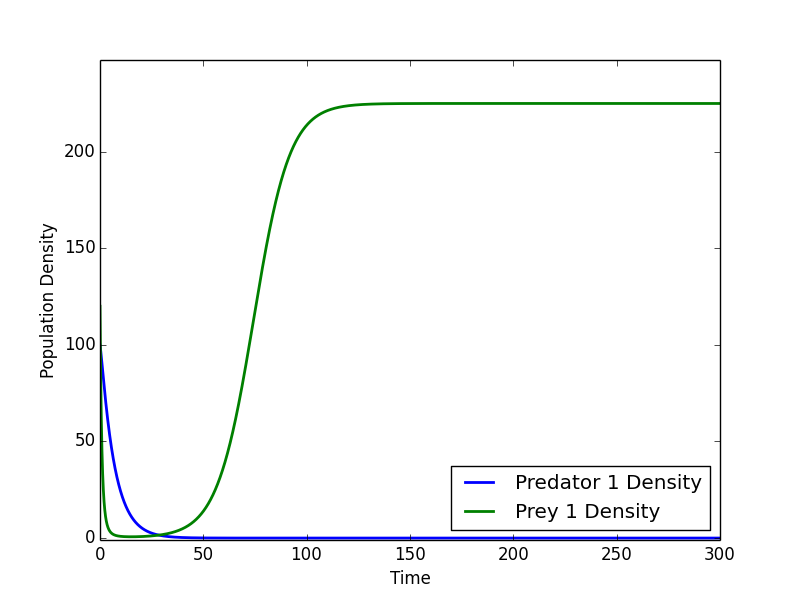
\includegraphics[width=5cm,height=3.75cm]{figures/1x1/variable_growth/stable_exclusion/densities.png}\\
			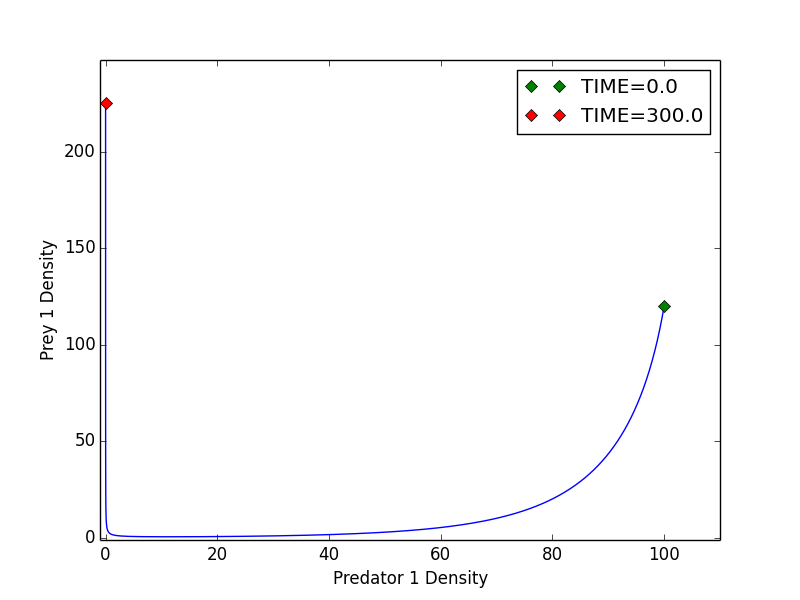
\includegraphics[width=5cm,height=3.75cm]{figures/1x1/variable_growth/stable_exclusion/density_phase_plane.png}
		\end{column}
		\begin{column}{.5\textwidth}
			\centering
			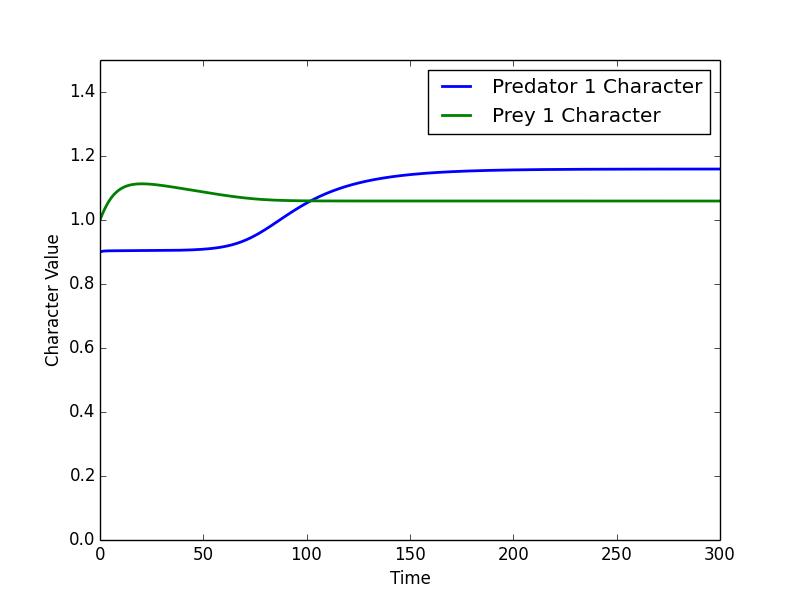
\includegraphics[width=5cm,height=3.75cm]{figures/1x1/variable_growth/stable_exclusion/traits.png}\\
			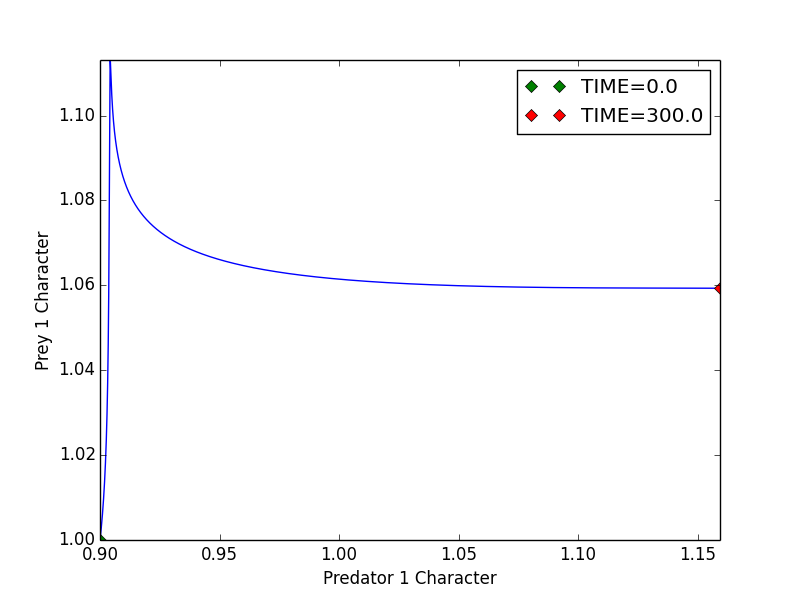
\includegraphics[width=5cm,height=3.75cm]{figures/1x1/variable_growth/stable_exclusion/trait_phase_plane.png}
		\end{column}
	\end{columns}
\end{frame}
\begin{frame}
	\frametitle{Figures - $1\times1$ - Stable Coexistence}
	\begin{columns}[t]
		\begin{column}{.5\textwidth}
			\centering
			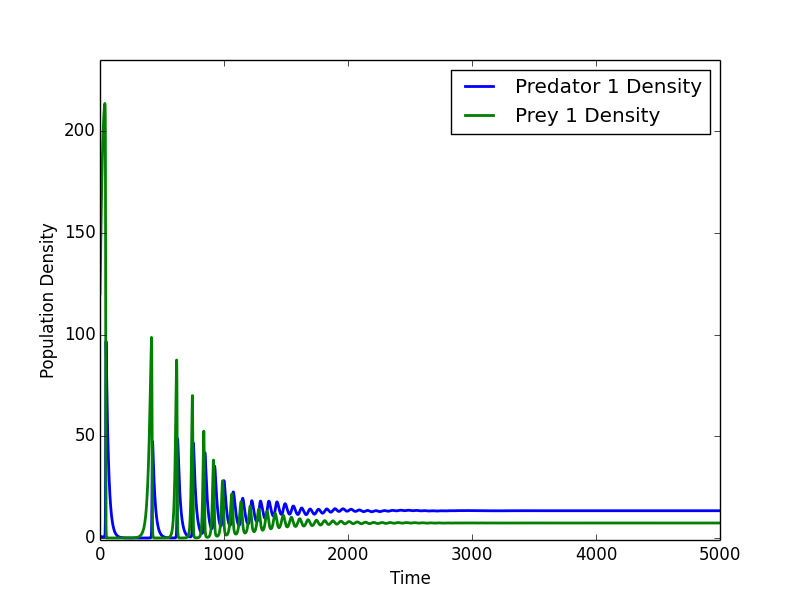
\includegraphics[width=5cm,height=3.75cm]{figures/1x1/variable_growth/stable_coexistence/densities.png}\\
			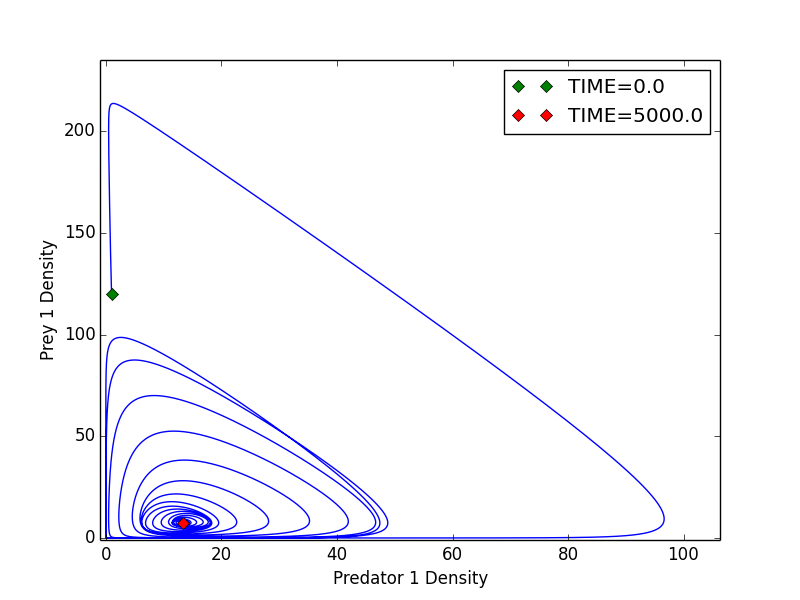
\includegraphics[width=5cm,height=3.75cm]{figures/1x1/variable_growth/stable_coexistence/density_phase_plane.png}
		\end{column}
		\begin{column}{.5\textwidth}
			\centering
			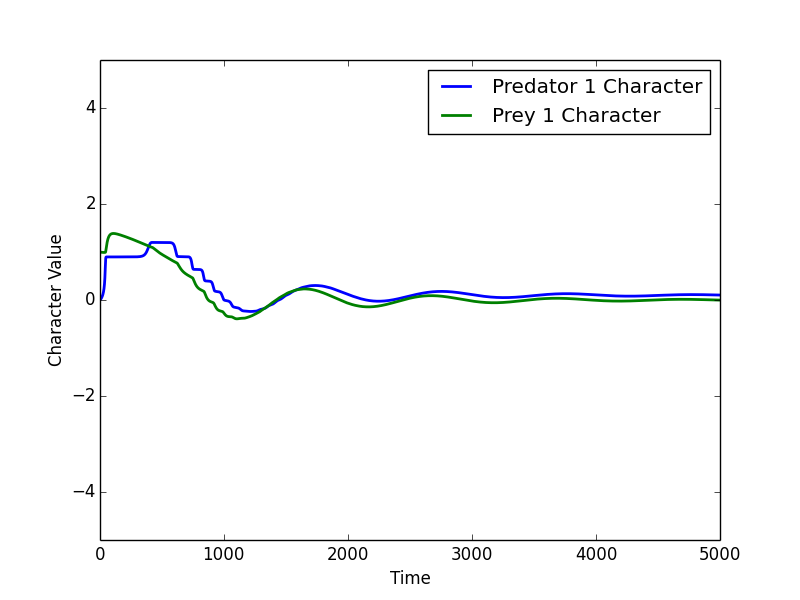
\includegraphics[width=5cm,height=3.75cm]{figures/1x1/variable_growth/stable_coexistence/traits.png}\\
			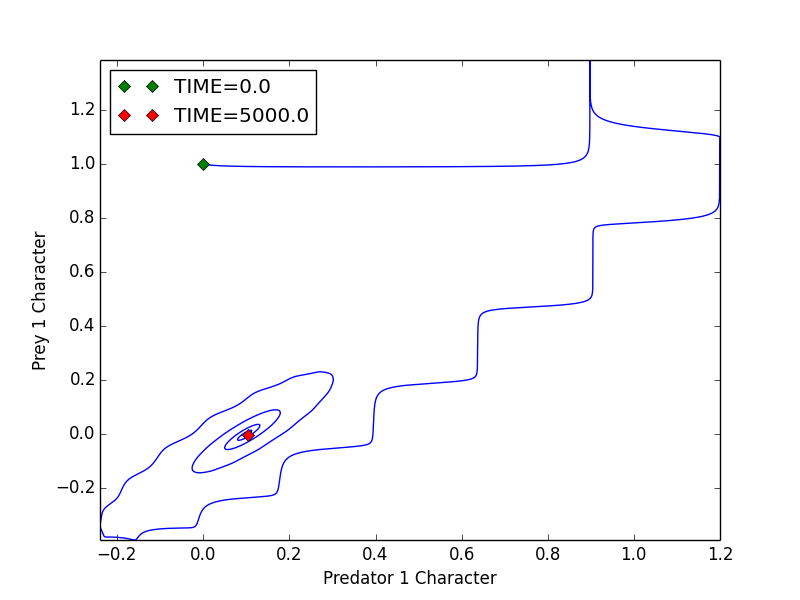
\includegraphics[width=5cm,height=3.75cm]{figures/1x1/variable_growth/stable_coexistence/trait_phase_plane.png}
		\end{column}
	\end{columns}
\end{frame}
\begin{frame}
	\frametitle{Figures - $1\times1$ - Stable Cycles {\normalsize(Red Queen Dynamics)}{\tiny[Kindrik, Kondrashov, 1994]}}
	\begin{columns}[t]
		\begin{column}{.5\textwidth}
			\centering
			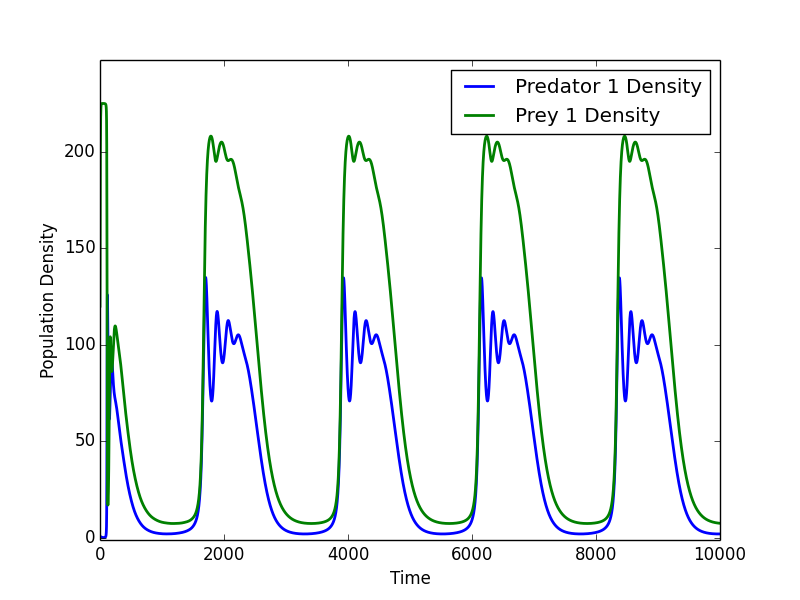
\includegraphics[width=5cm,height=3.75cm]{figures/1x1/variable_growth/stable_cycles/densities.png}\\
			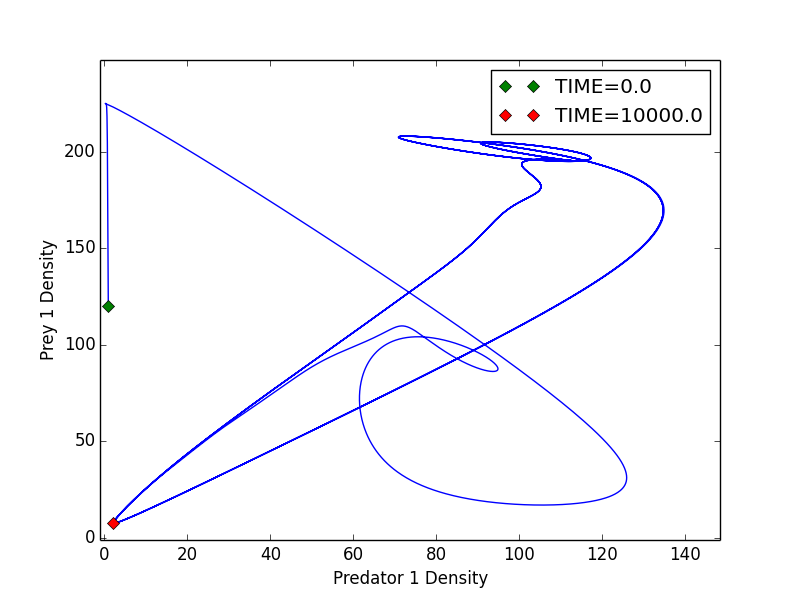
\includegraphics[width=5cm,height=3.75cm]{figures/1x1/variable_growth/stable_cycles/density_phase_plane.png}
		\end{column}
		\begin{column}{.5\textwidth}
			\centering
			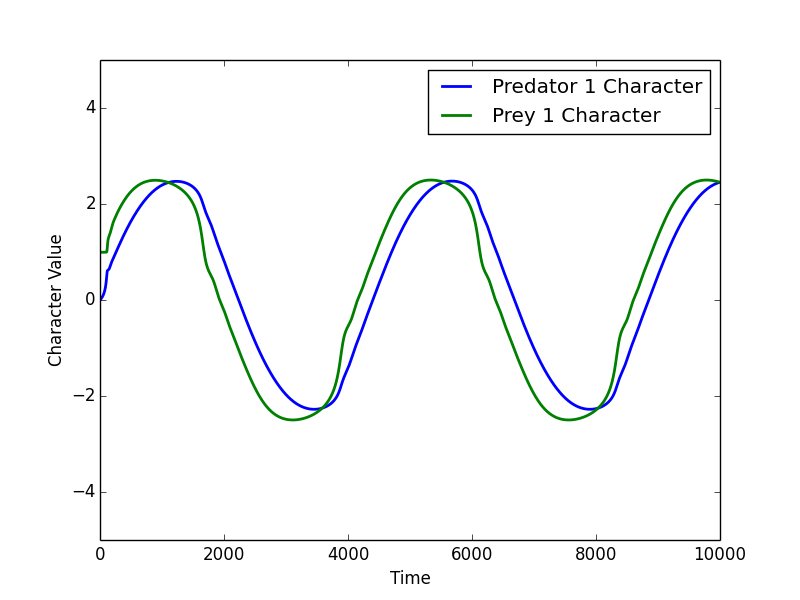
\includegraphics[width=5cm,height=3.75cm]{figures/1x1/variable_growth/stable_cycles/traits.png}\\
			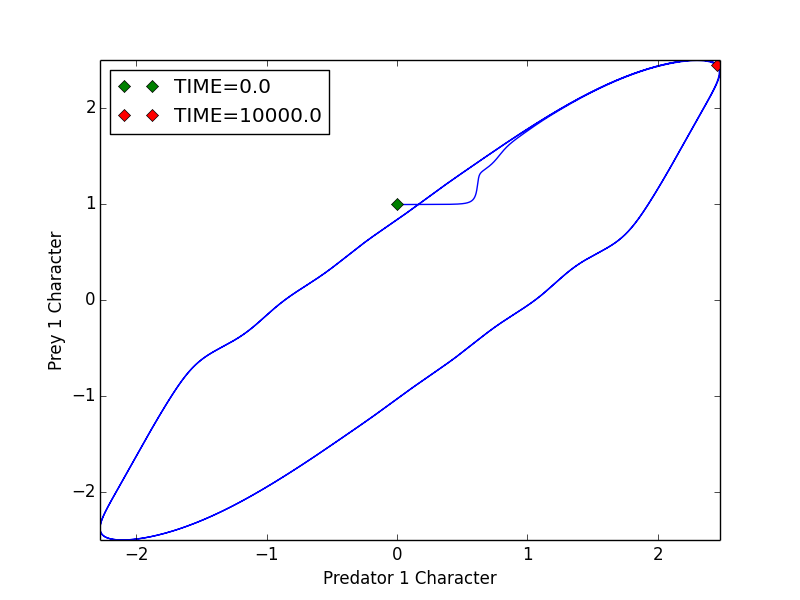
\includegraphics[width=5cm,height=3.75cm]{figures/1x1/variable_growth/stable_cycles/trait_phase_plane.png}
		\end{column}
	\end{columns}
\end{frame}

% \begin{frame}
% 	\LARGE \vspace{-20pt}
% 	\begin{center}
% 		\underline{\it Question}\\
% 		What happens when the exclusion {\bf AND} coexistence stability criterion are {\bf NOT} met? \\ \vspace{15pt}
% 		\uncover<2->{
% 		\underline{\it Answer}\\
% 		{\bf Stable Limit Cycles}}
% 	\end{center}
% \end{frame}

\begin{frame}
	\frametitle{Contour Plot - Coexistence Asymptotic Stability Criterion}
	\vspace{-5pt}
	\begin{center}
		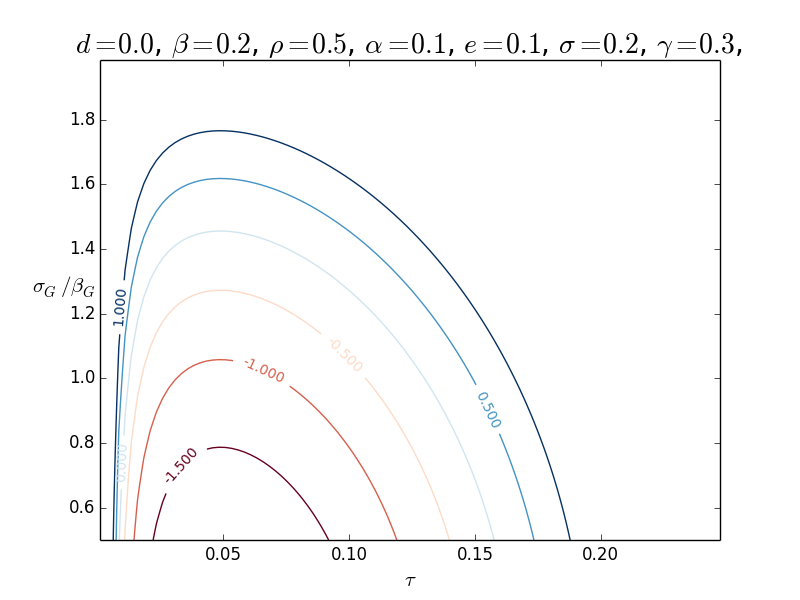
\includegraphics[width=8cm, height=5cm]{figures/1x1/variable_growth/contour_plots/tau_ratio_150417_125636.png} \\
	\end{center}
	\vspace{-10pt}
	\begin{align*}
		f_{\text{stable}}(\text{\it system parameters}) = \dfrac{\sigma_G^2}{\beta_G^2} -\dfrac{\rho\gamma}{d\sqrt{B}}\left(1 - \dfrac{d\sqrt{A}}{Ke\alpha\tau}\right)\left(1 - \dfrac{A}{B}\right)
	\end{align*}
	$f_{\text{stable}} > 0 \implies \text{Coexistence is \it stable}$ \\
	$f_{\text{stable}} < 0 \implies \text{Coexistence is \it unstable}$ \\
	$f_{\text{stable}} = 0 \implies \text{Hopf Bifurcation}$
\end{frame}
\begin{frame}
	\frametitle{{\small$\tau = 0.05$:}\ \ \ \ Limit Cycle\ \ \ \ \ \ \ \ vs.\ \ \ \ \ \ \ \ \ \ \ \ Node}
	\begin{columns}[t]
		\begin{column}{.5\textwidth}
			\centering
			$\frac{\sigma_G}{\beta_G} = 1.3 \implies f_{\text{stable}} < 0$\\
			\vspace{-1pt}
			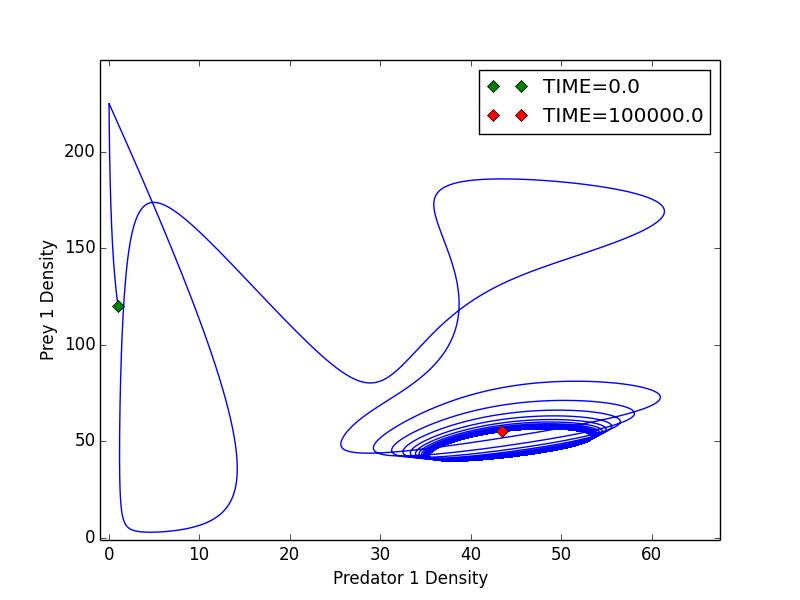
\includegraphics[width=5cm,height=3.55cm]{figures/1x1/variable_growth/contour_plots/density_phase_plane_limit_cycle.png}\\
			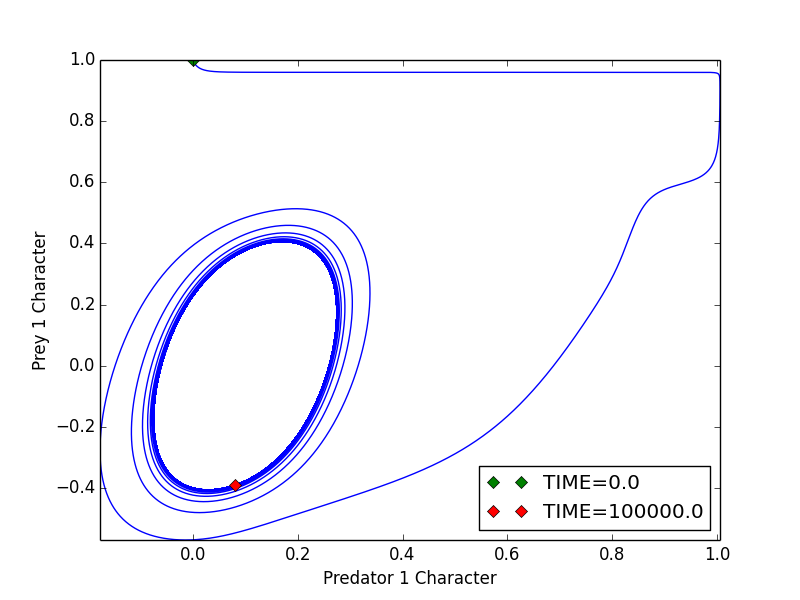
\includegraphics[width=5cm,height=3.55cm]{figures/1x1/variable_growth/contour_plots/trait_phase_plane_limit_cycle.png}
		\end{column}
		\hspace{-30pt}
		\vrule{}
		\begin{column}{.5\textwidth}
			\centering
			$\frac{\sigma_G}{\beta_G} = 1.5 \implies f_{\text{stable}} > 0$\\
			\vspace{-1pt}
			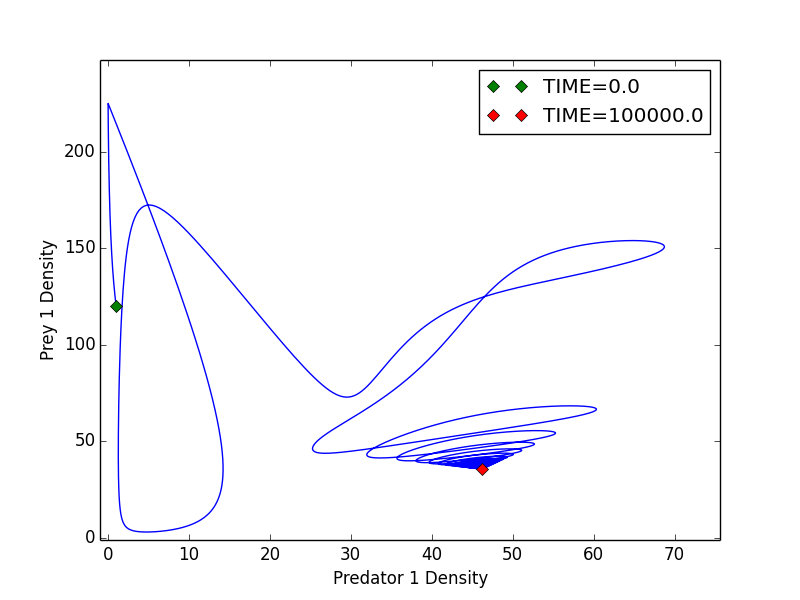
\includegraphics[width=5cm,height=3.55cm]{figures/1x1/variable_growth/contour_plots/density_phase_plane_node.png}\\
			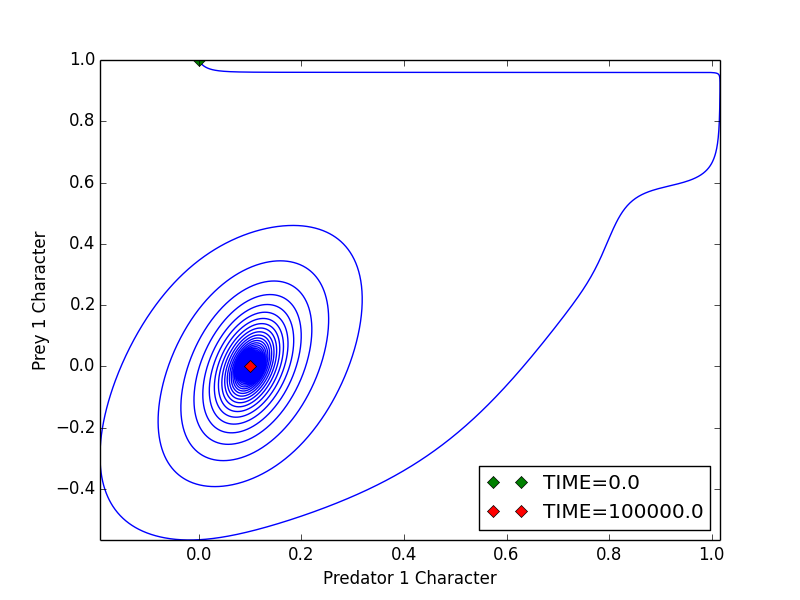
\includegraphics[width=5cm,height=3.55cm]{figures/1x1/variable_growth/contour_plots/trait_phase_plane_node.png}
		\end{column}
	\end{columns}
\end{frame}

\section{Discussion}
\subsection{Summary of the $1\times 1$ Model}
\begin{frame}
	\frametitle{Summary of the $1\times 1$ Model}
	\begin{itemize}
		\item 4-dimensional system of ODEs
		\begin{itemize}
			\item 2 ODEs describing the change in {\bf population size} over time
			\item 2 ODEs describing the change in {\bf trait value} over time
		\end{itemize}
		\uncover<2->{\item 3 equilibrium points
		\begin{itemize}
			\item Extinction (Unstable)
			\item Exclusion (Stable under certain conditions)
			\item Coexistence (Stable under certain conditions)
		\end{itemize}}
		\uncover<3->{\item Non-Equilibrium Dynamics
		\begin{itemize}
			\item Constant Growth Rate
			\begin{itemize}
				\item ``Arms Race'' Coexistence
			\end{itemize}
			\item Gaussian Growth Rate Function
			\begin{itemize}
				\item Stable Limit Cycles
			\end{itemize}
		\end{itemize}}
	\end{itemize}
\end{frame}

\subsection*{General Ditrophic Expansion}
\begin{frame}
	\frametitle{Expansion of Fitness Functions}
	{\bf Prey Fitness}
	\begin{align*}
		{\color{blue}Y(N, n, M, m)} &= r(n)\left(1 - \frac{N}{K}\right) - Ma(n, m) \\
		\uncover<2->{\scriptsize&\downarrow} \\
		\uncover<2->{{\color{blue}Y_j(N_j, n_j, [M_i]_{i=1}^{u}, [m_i]_{i=1}^{u})} &= r_j(n_j)\left(1 - \frac{N_j}{K_j}\right) - \sum\limits_{i = 1}^{u}M_ia_{ij}(n_j, m_i)}
	\end{align*}
	{\bf Predator Fitness}
	\begin{align*}
		{\color{red}W(N, n, M, m)} &= eNa(n, m) - d \\
		\uncover<3->{\scriptsize&\downarrow} \\
		\uncover<3->{{\color{red}W_i([N_j]_{j=1}^{v}, [n_j]_{j=1}^{v}, M_i, m_i)} &= \sum\limits_{j = 1}^{v}\Big[e_{ij}N_ja_{ij}(n_j, m_i)\Big] - d_i}
	\end{align*}
	\uncover<2->{\begin{center}{\bf Notation:} $[x_i]_{i=1}^{u} = x_1, \dots, x_u$\end{center}}
\end{frame}
\begin{frame}
	\frametitle{Average Fitness Calculation}
	\begin{align*}
		{\color{blue}\overline{Y}_j(N_j, \overline{n_j}, [M_i]_{i=1}^{u}, }&{\color{blue}[\overline{m_i}]_{i=1}^{u})} \\
		&= \int\limits_{\mathbb{R}^{u+1}} Y_j \cdot \prod\limits_{i=1}^{u}\Big[p_i(m_i, \overline{m_i})\Big] \cdot p(n, \overline{n}) \prod\limits_{i=1}^{u}\Big[dm_i\Big] dn_j\\
		&= {\color{blue}\overline{r_j}(\overline{n_j})\left(1 - \frac{N_j}{K_j}\right) - \sum\limits_{i = 1}^{u}M_i\overline{a_{ij}}(\overline{n_j}, \overline{m_i})}
	\end{align*}
	\begin{align*}
		{\color{red}\overline{W}_i(N_j, \overline{n_j}, [M_i]_{i=1}^{u}, }&{\color{red}[\overline{m_i}]_{i=1}^{u})} \\
		&= \int\limits_{\mathbb{R}^{u+1}} W_i \cdot p_i(m_i, \overline{m_i}) \cdot \prod\limits_{j=1}^{v}\Big[p(n_j, \overline{n_j})\Big] dm_i \prod\limits_{j=1}^{v}\Big[dn_j\Big]\\
		&= {\color{red}\sum\limits_{j = 1}^{v}\Big[e_{ij}N_j\overline{a_{ij}}(\overline{n_j}, \overline{m_i})\Big] - d_i}
	\end{align*}
\end{frame}
\begin{frame}
	\frametitle{The Complete $v\times u$ Model - \normalsize($v$ Prey Species, $u$ Predator Species)}
	{\bf Ecological Components}
	\begin{align*}
		\frac{dN_j}{dt} &= N_j{\color{blue}\overline{Y_j}} = N_j {\color{blue}\left[{\color{blue}\overline{r_j}(\overline{n_j})\left(1 - \frac{N_j}{K_j}\right) - \sum\limits_{i = 1}^{u}M_i\overline{a_{ij}}(\overline{n_j}, \overline{m_i})}\right]} \\
		\frac{dM_i}{dt} &= M_i{\color{red}\overline{W_i}} = M_i {\color{red}\left[\sum\limits_{j = 1}^{v}\Big[e_{ij}N_j\overline{a_{ij}}(\overline{n_j}, \overline{m_i})\Big] - d_i\right]}
	\end{align*}
	{\bf Evolutionary Components}
	\begin{align*}
		\frac{d\overline{n_j}}{dt} &= \beta_{Gj}^2{\color{cyan}\frac{\partial \overline{Y_j}}{\partial \overline{n_j}}} = \beta_{Gj}^2{\color{cyan}\left[\overline{r_j}(\overline{n_j})\left(1 - \frac{N_j}{K_j}\right)\frac{(\phi_j - \overline{n_j})}{\beta_j^2 + \gamma_j^2}\right.}
		\\&\hphantom{\text{mmmmmmmmmmm}}{\left.\color{cyan}+ \sum\limits_{i=1}^{u}\left[\frac{M_i(\theta_{ij} - (\overline{m_i} - \overline{n_j}))}{\sigma_i^2 + \beta_j^2 + \tau_{ij}^2} \overline{a_{ij}}(\overline{n_j}, \overline{m_i})\right]\right]}\\
		\frac{d\overline{m_i}}{dt} &= \sigma_{Gi}^2{\color{magenta}\frac{\partial\overline{W_i}}{\partial\overline{m_i}}} = \sigma_{Gi}^2{\color{magenta}\sum\limits_{j=1}^{v}\left[\frac{e_{ij}N_j(\theta_{ij} - (\overline{m_i} - \overline{n_j}))}{\sigma_i^2 + \beta_j^2 + \tau_{ij}^2} \overline{a_{ij}}(\overline{n_j}, \overline{m_i})\right]}
	\end{align*}
\end{frame}
\begin{frame}
	\frametitle{The Complete $v\times u$ Model - \normalsize($v$ Prey Species, $u$ Predator Species)}
	\Wider[6em]{
	\begin{center}
		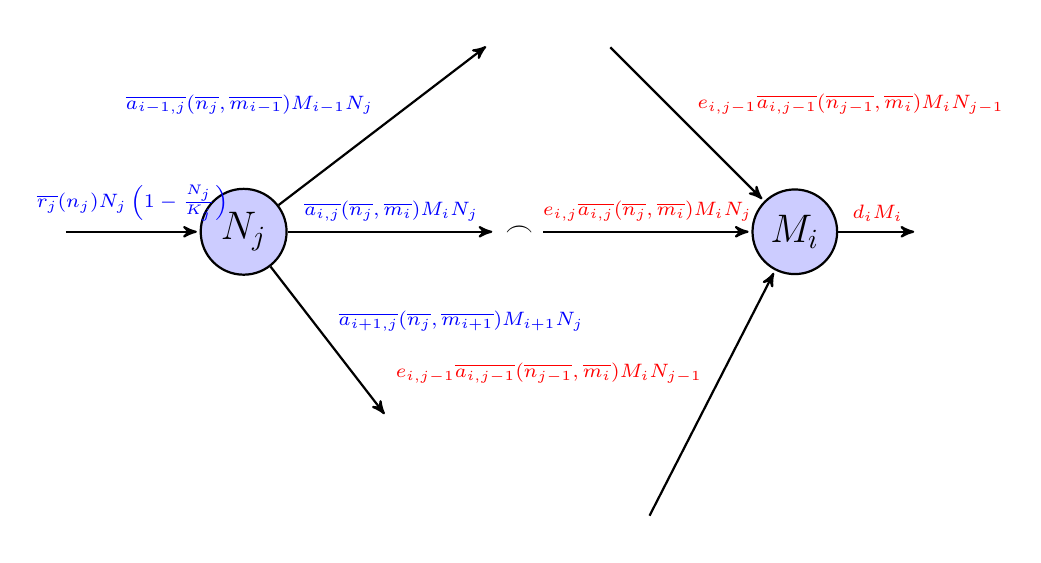
\begin{tikzpicture}[->,>=stealth',shorten >=1pt,auto,node distance=3.5cm, thick,main node/.style={circle,fill=blue!20,draw,font=\sffamily\Large\bfseries}]
	
			\node[main node] (n1) {$N_j$};
			\node (midpt1) [right of=n1] {$\frown$};
			\node[main node] (m1) [right of=midpt1] {$M_i$};
			\node (input1) [left =1.7cm of n1] {};
			\node (output1) [right = 1cm of m1] {};
			\node (upright) [above right of=n1] {};
			\node (furtherright) [right = .5cm of upright] {};
			\node (downright) [below right of=n1] {};
			\node (alittleleft) [left = 0.3cm of downright] {};
			\node (upleft) [above left of=m1] {};
			\node (downleft) [below left of=m1] {};
			\node (furtherdown) [below = 1cm of downleft] {};
			\node (alittleright) [right = 0.3cm of furtherdown] {};
	
			\path[every node/.style={font=\sffamily\small}]
			(input1)	edge node {\scriptsize{\color{blue}$\overline{r_j}(n_j)N_j\left(1 - \frac{N_j}{K_j}\right)$}} (n1)
			(n1)		edge node {\scriptsize{\color{blue}$\overline{a_{i,j}}(\overline{n_j}, \overline{m_i})M_iN_j$}} (midpt1)
					edge node {\scriptsize{\color{blue}$\overline{a_{i-1,j}}(\overline{n_j}, \overline{m_{i-1}})M_{i-1}N_j$}} (furtherright)
					edge node {\scriptsize{\color{blue}$\overline{a_{i+1,j}}(\overline{n_j}, \overline{m_{i+1}})M_{i+1}N_j$}} (alittleleft)
			(midpt1)	edge node {\scriptsize{\color{red}$e_{i,j}\overline{a_{i,j}}(\overline{n_j}, \overline{m_i})M_iN_j$}} (m1)
			(m1)		edge node {\scriptsize{\color{red}$d_iM_i$}} (output1)
			(upleft)	edge node {\scriptsize{\color{red}$e_{i,j-1}\overline{a_{i,j-1}}(\overline{n_{j-1}}, \overline{m_i})M_iN_{j-1}$}} (m1)
			(alittleright)	edge node {\scriptsize{\color{red}$e_{i,j-1}\overline{a_{i,j-1}}(\overline{n_{j-1}}, \overline{m_i})M_iN_{j-1}$}} (m1)
			;
		\end{tikzpicture}\vskip0.35cm
	\end{center}
	}
\end{frame}

\subsection{$2\times 1$ and $1\times 2$ Simulations}

\begin{frame}
	\frametitle{The Complete $2\times 1$ Model - \normalsize($2$ Prey Species, $1$ Predator Species)}
	{\bf Ecological Components}
	{\footnotesize\begin{align*}
		\frac{dN_1}{dt} &= N_1{\color{blue}\overline{Y_1}} = N_1 {\color{blue}\left[{\color{blue}\overline{r_1}(\overline{n_1})\left(1 - \frac{N_1}{K_1}\right) - M\overline{a_1}(\overline{n_1}, \overline{m})}\right]} \\
		\frac{dN_2}{dt} &= N_2{\color{blue}\overline{Y_2}} = N_2 {\color{blue}\left[{\color{blue}\overline{r_2}(\overline{n_2})\left(1 - \frac{N_2}{K_2}\right) - M\overline{a_2}(\overline{n_2}, \overline{m})}\right]} \\
		\frac{dM}{dt} &= M{\color{red}\overline{W}} = M {\color{red}\left[\sum\limits_{j = 1}^{2}\Big[e_{j}N_j\overline{a_j}(\overline{n_j}, \overline{m})\Big] - d\right]}
	\end{align*}}%
	{\bf Evolutionary Components}
	{\footnotesize\begin{align*}
		\frac{d\overline{n_1}}{dt} &= \beta_{G1}^2{\color{cyan}\frac{\partial \overline{Y_1}}{\partial \overline{n_1}}} = \beta_{G1}^2{\color{cyan}\left[\overline{r_1}(\overline{n_1})\left(1 - \frac{N_1}{K_1}\right)\frac{(\phi_1 - \overline{n_1})}{\beta_1^2 + \gamma_1^2} + \frac{M(\theta_{1} - (\overline{m} - \overline{n_1}))}{\sigma^2 + \beta_1^2 + \tau_{1}^2} \overline{a_1}(\overline{n_1}, \overline{m})\right]}\\
		\frac{d\overline{n_2}}{dt} &= \beta_{G1}^2{\color{cyan}\frac{\partial \overline{Y_2}}{\partial \overline{n_2}}} = \beta_{G2}^2{\color{cyan}\left[\overline{r_2}(\overline{n_2})\left(1 - \frac{N_2}{K_2}\right)\frac{(\phi_2 - \overline{n_2})}{\beta_2^2 + \gamma_2^2} + \frac{M(\theta_{2} - (\overline{m} - \overline{n_2}))}{\sigma^2 + \beta_2^2 + \tau_{2}^2} \overline{a_2}(\overline{n_2}, \overline{m})\right]}\\
		\frac{d\overline{m}}{dt} &= \sigma_{G}^2{\color{magenta}\frac{\partial\overline{W}}{\partial\overline{m}}} = \sigma_{G}^2{\color{magenta}\sum\limits_{j=1}^{2}\left[\frac{e_{j}N_j(\theta_{j} - (\overline{m} - \overline{n_j}))}{\sigma^2 + \beta_j^2 + \tau_{j}^2} \overline{a_j}(\overline{n_j}, \overline{m})\right]}
	\end{align*}}%
\end{frame}
\begin{frame}
	\frametitle{Figures - $2\times1$}
	\begin{columns}[t]
		\begin{column}{.5\textwidth}
			\centering
			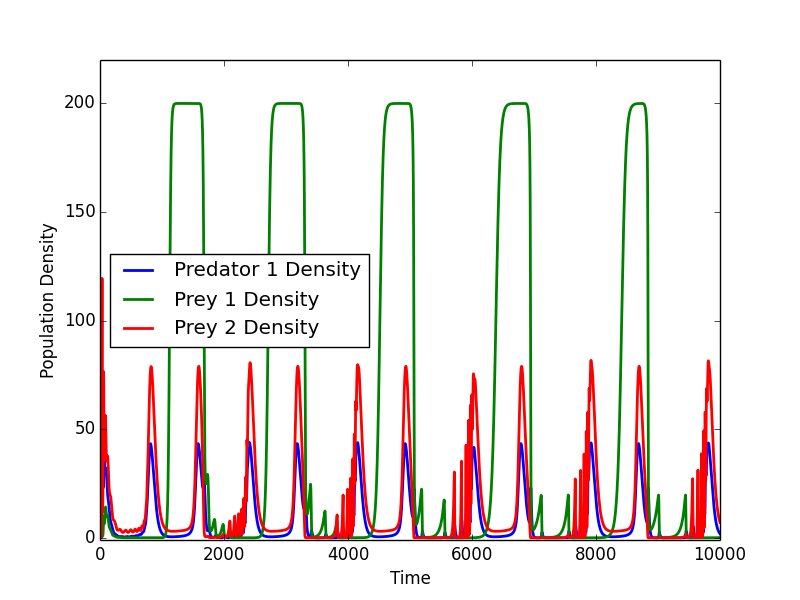
\includegraphics[width=5cm,height=3.75cm]{figures/1x2/variable_growth/densities_cyclic_domination.png}\\
			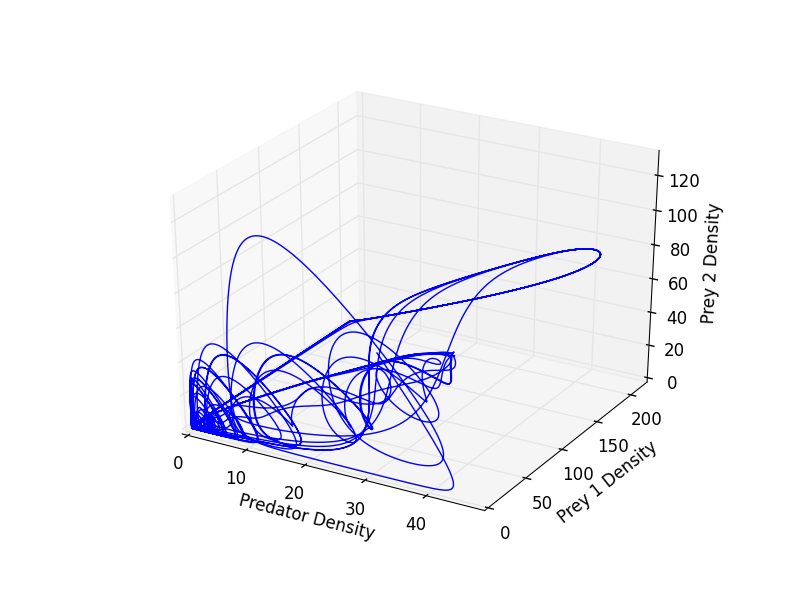
\includegraphics[width=5cm,height=3.75cm]{figures/1x2/variable_growth/density_phase_plane_cyclic_domination.png}
		\end{column}
		\begin{column}{.5\textwidth}
			\centering
			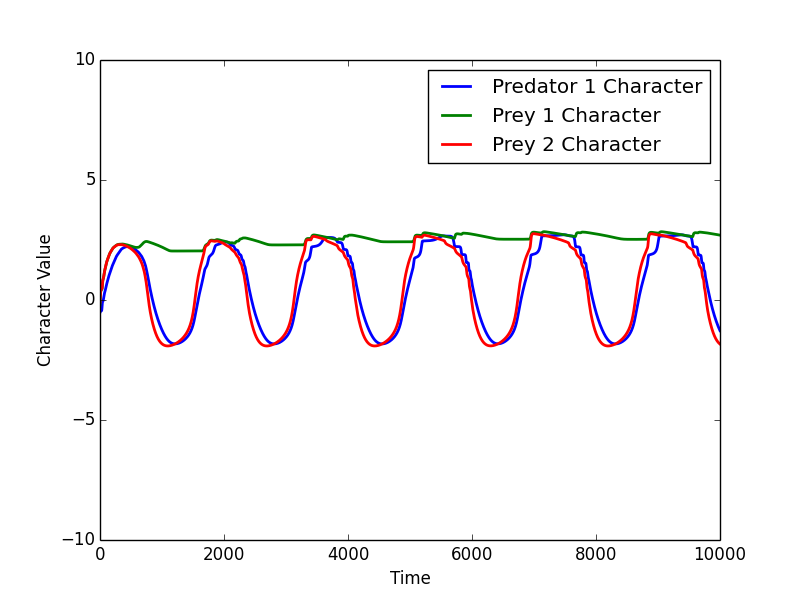
\includegraphics[width=5cm,height=3.75cm]{figures/1x2/variable_growth/traits_cyclic_domination.png}\\
			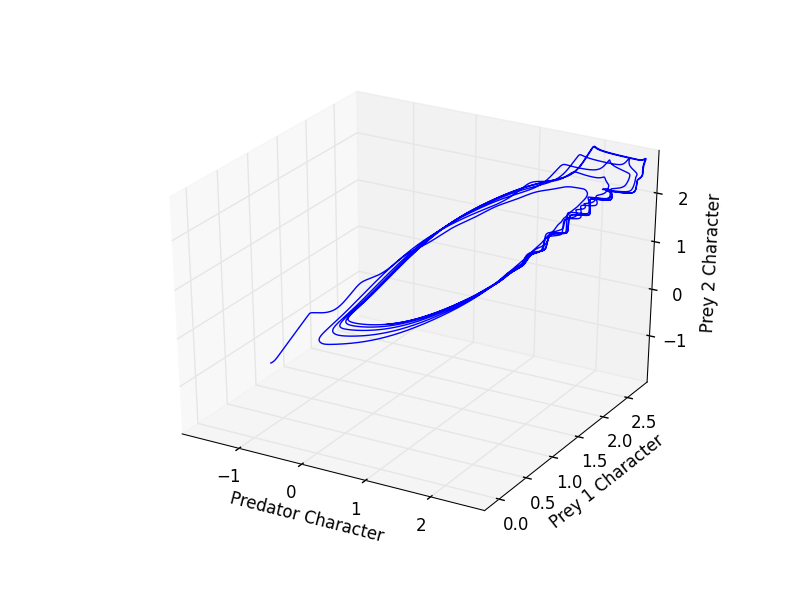
\includegraphics[width=5cm,height=3.75cm]{figures/1x2/variable_growth/trait_phase_plane_cyclic_domination.png}
		\end{column}
	\end{columns}
\end{frame}
\begin{frame}
	\frametitle{Figures - $2\times1$}
	\begin{columns}[t]
		\begin{column}{.5\textwidth}
			\centering
			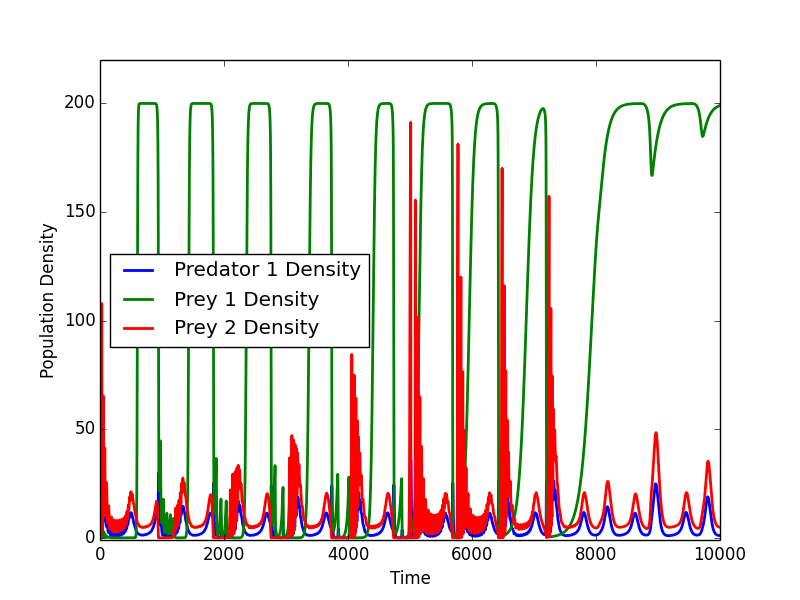
\includegraphics[width=5cm,height=3.75cm]{figures/1x2/variable_growth/densities_stable_domination.png}\\
			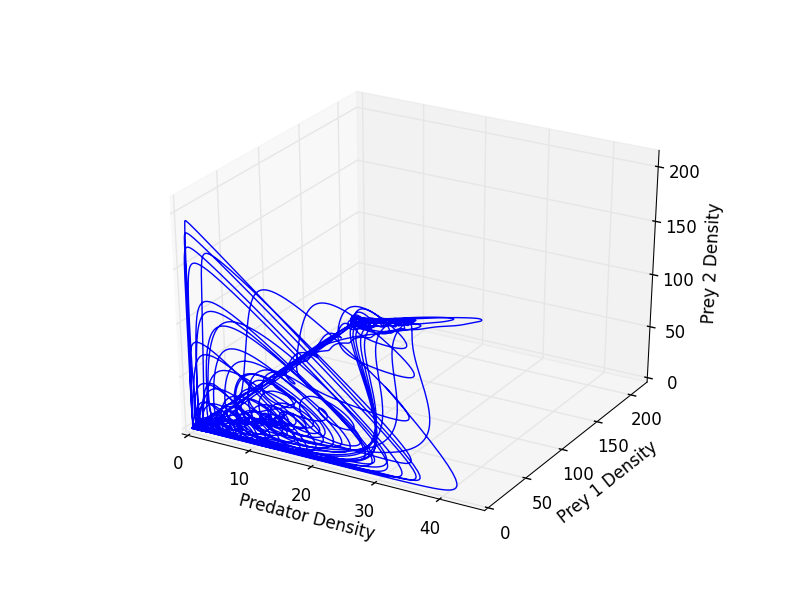
\includegraphics[width=5cm,height=3.75cm]{figures/1x2/variable_growth/density_phase_plane_stable_domination.png}
		\end{column}
		\begin{column}{.5\textwidth}
			\centering
			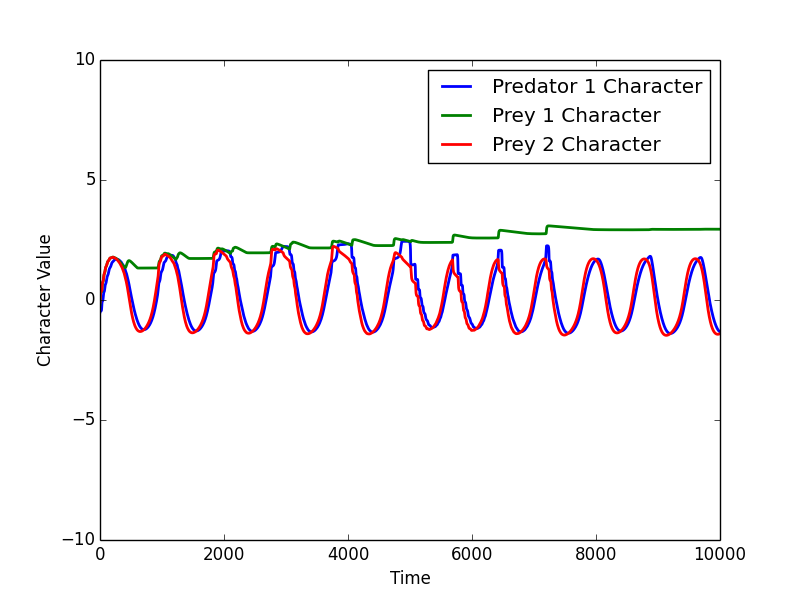
\includegraphics[width=5cm,height=3.75cm]{figures/1x2/variable_growth/traits_stable_domination.png}\\
			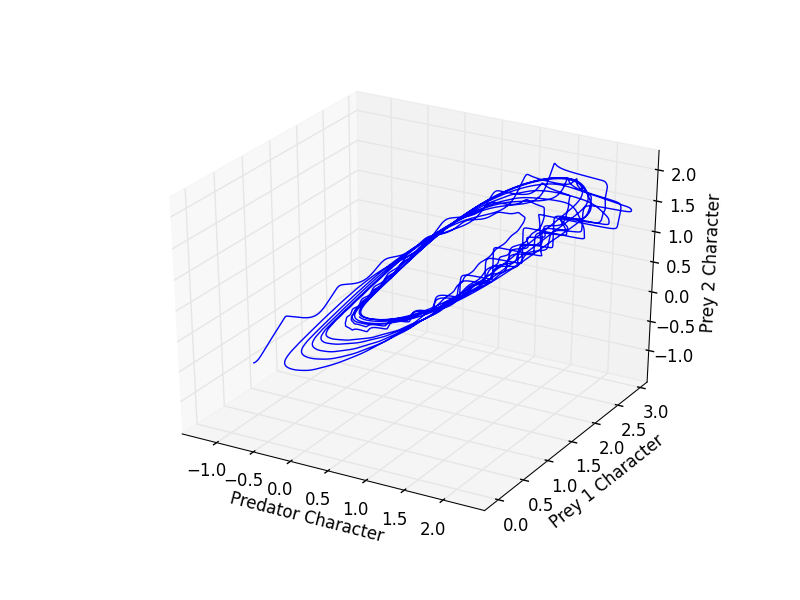
\includegraphics[width=5cm,height=3.75cm]{figures/1x2/variable_growth/trait_phase_plane_stable_domination.png}
		\end{column}
	\end{columns}
\end{frame}
\begin{frame}
	\frametitle{Figures - $2\times1$}
	\begin{columns}[t]
		\begin{column}{.5\textwidth}
			\centering
			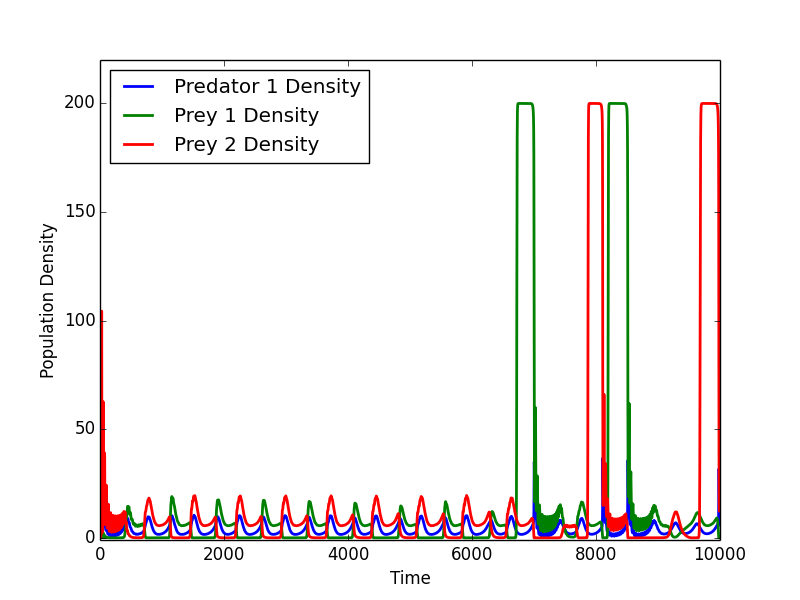
\includegraphics[width=5cm,height=3.75cm]{figures/1x2/variable_growth/densities_random_domination.png}\\
			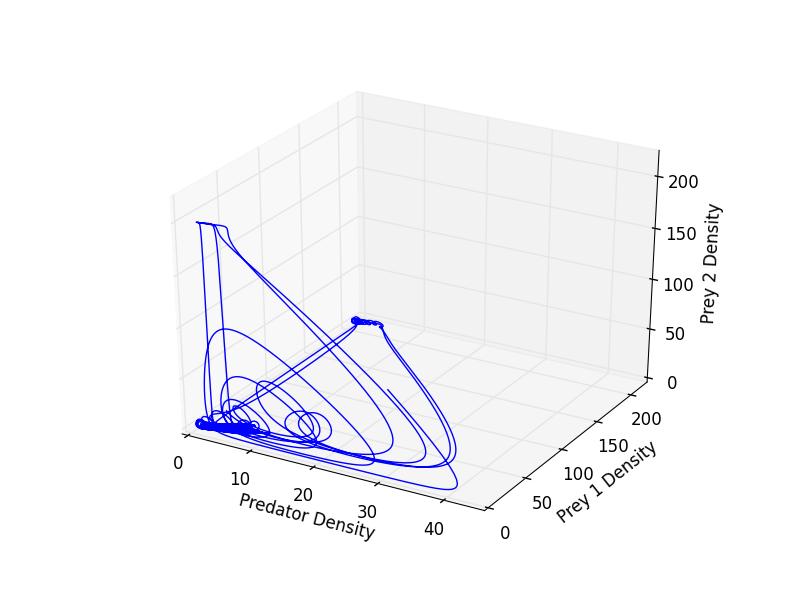
\includegraphics[width=5cm,height=3.75cm]{figures/1x2/variable_growth/density_phase_plane_random_domination.png}
		\end{column}
		\begin{column}{.5\textwidth}
			\centering
			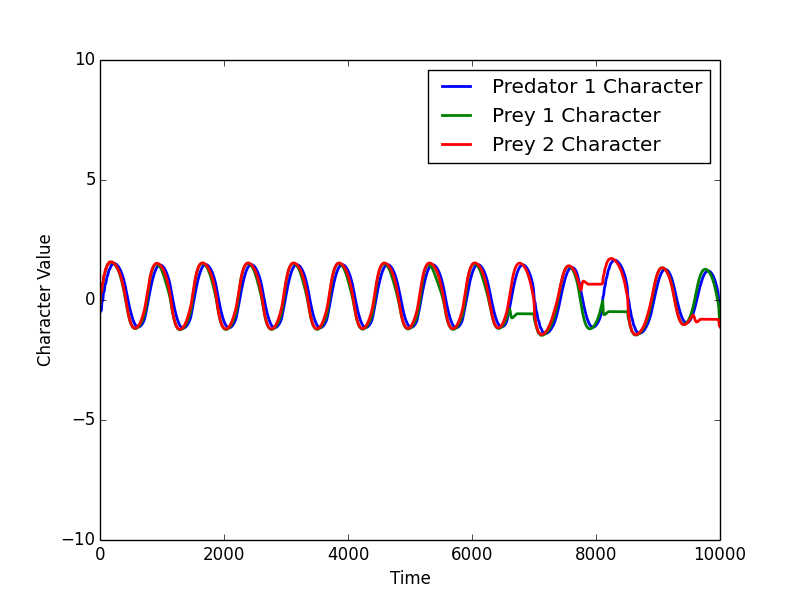
\includegraphics[width=5cm,height=3.75cm]{figures/1x2/variable_growth/traits_random_domination.png}\\
			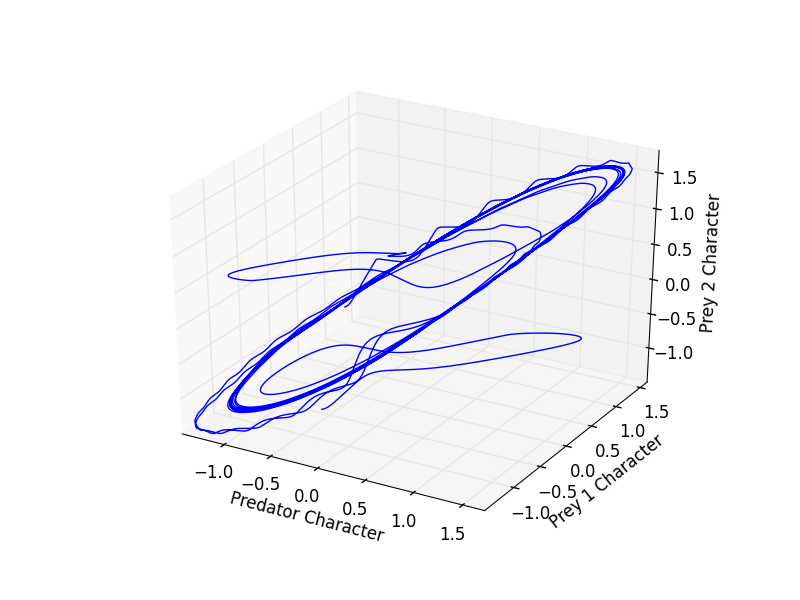
\includegraphics[width=5cm,height=3.75cm]{figures/1x2/variable_growth/trait_phase_plane_random_domination.png}
		\end{column}
	\end{columns}
\end{frame}
\begin{frame}
	\frametitle{Figures - $2\times1$}
	\begin{columns}[t]
		\begin{column}{.5\textwidth}
			\centering
			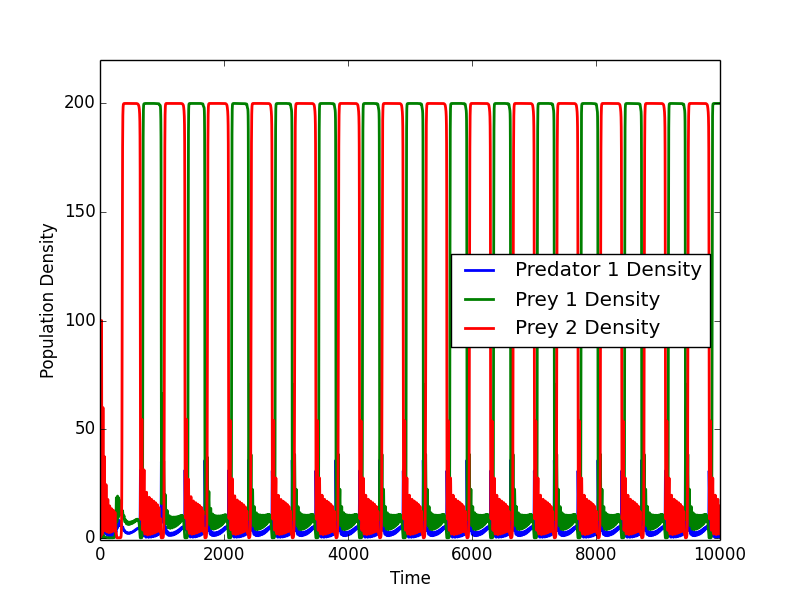
\includegraphics[width=5cm,height=3.75cm]{figures/1x2/variable_growth/densities_RQD.png}\\
			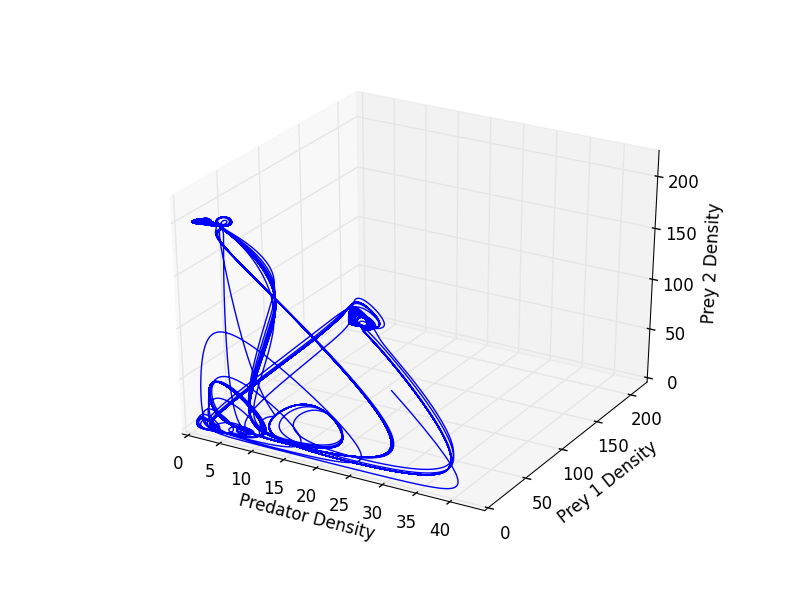
\includegraphics[width=5cm,height=3.75cm]{figures/1x2/variable_growth/density_phase_plane_RQD.png}
		\end{column}
		\begin{column}{.5\textwidth}
			\centering
			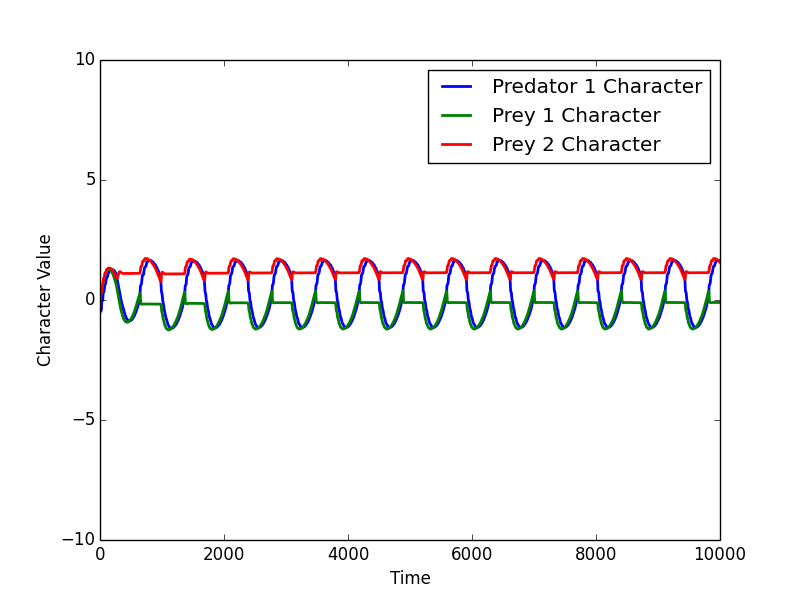
\includegraphics[width=5cm,height=3.75cm]{figures/1x2/variable_growth/traits_RQD.png}\\
			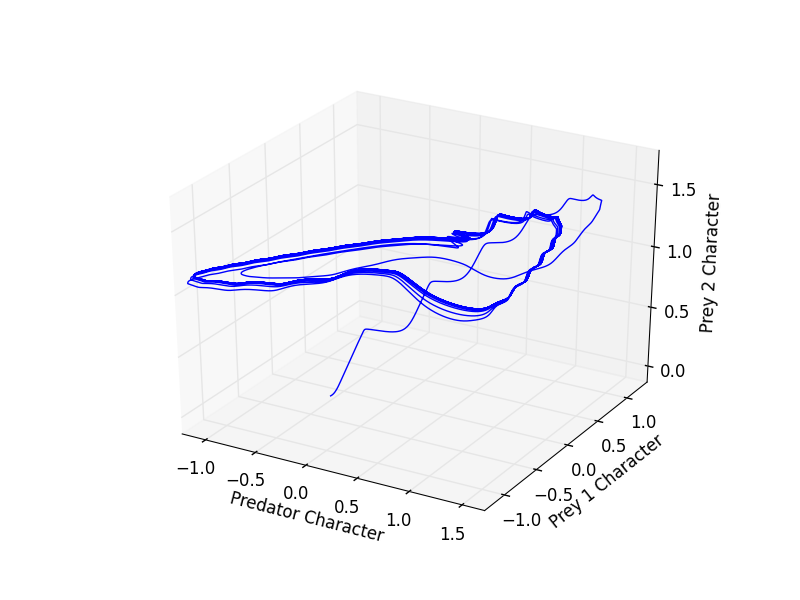
\includegraphics[width=5cm,height=3.75cm]{figures/1x2/variable_growth/trait_phase_plane_RQD.png}
		\end{column}
	\end{columns}
\end{frame}

\begin{frame}
	\frametitle{The Complete $1\times 2$ Model - \normalsize($1$ Prey Species, $2$ Predator Species)}
	{\bf Ecological Components}
	{\footnotesize\begin{align*}
		\frac{dN}{dt} &= N{\color{blue}\overline{Y}} = N {\color{blue}\left[{\color{blue}\overline{r}(\overline{n})\left(1 - \frac{N}{K}\right) - \sum\limits_{i=1}^2M_i\overline{a_i}(\overline{n}, \overline{m_i})}\right]} \\
		\frac{dM_1}{dt} &= M_1{\color{red}\overline{W}} = M_1 {\color{red}\Big[e_{1}N\overline{a_1}(\overline{n}, \overline{m_1}) - d_1\Big]} \\
		\frac{dM_2}{dt} &= M_2{\color{red}\overline{W}} = M_2 {\color{red}\Big[e_{2}N\overline{a_2}(\overline{n}, \overline{m_2}) - d_2\Big]}
	\end{align*}}%
	{\bf Evolutionary Components}
	{\footnotesize\begin{align*}
		\frac{d\overline{n}}{dt} &= \beta_{G}^2{\color{cyan}\frac{\partial \overline{Y}}{\partial \overline{n}}} = \beta_{G}^2{\color{cyan}\left[\overline{r}(\overline{n})\left(1 - \frac{N}{K}\right)\frac{(\phi - \overline{n})}{\beta^2 + \gamma^2} + \sum\limits_{i=1}^{2}\left[\frac{M_i(\theta_{i} - (\overline{m_i} - \overline{n}))}{\sigma_i^2 + \beta^2 + \tau_{i}^2} \overline{a_{i}}(\overline{n}, \overline{m_i})\right]\right]}\\
		\frac{d\overline{m_1}}{dt} &= \sigma_{G1}^2{\color{magenta}\frac{\partial\overline{W_1}}{\partial\overline{m_1}}} = \sigma_{G1}^2{\color{magenta}\left[\frac{e_{1}N(\theta_{1} - (\overline{m_1} - \overline{n}))}{\sigma_1^2 + \beta^2 + \tau_{1}^2} \overline{a_1}(\overline{n}, \overline{m_1})\right]} \\
		\frac{d\overline{m_2}}{dt} &= \sigma_{G1}^2{\color{magenta}\frac{\partial\overline{W_2}}{\partial\overline{m_2}}} = \sigma_{G1}^2{\color{magenta}\left[\frac{e_{2}N(\theta_{2} - (\overline{m_2} - \overline{n}))}{\sigma_2^2 + \beta^2 + \tau_{2}^2} \overline{a_2}(\overline{n}, \overline{m_2})\right]}
	\end{align*}}%
\end{frame}
\begin{frame}
	\frametitle{Figures - $1\times2$}
	\begin{columns}[t]
		\begin{column}{.5\textwidth}
			\centering
			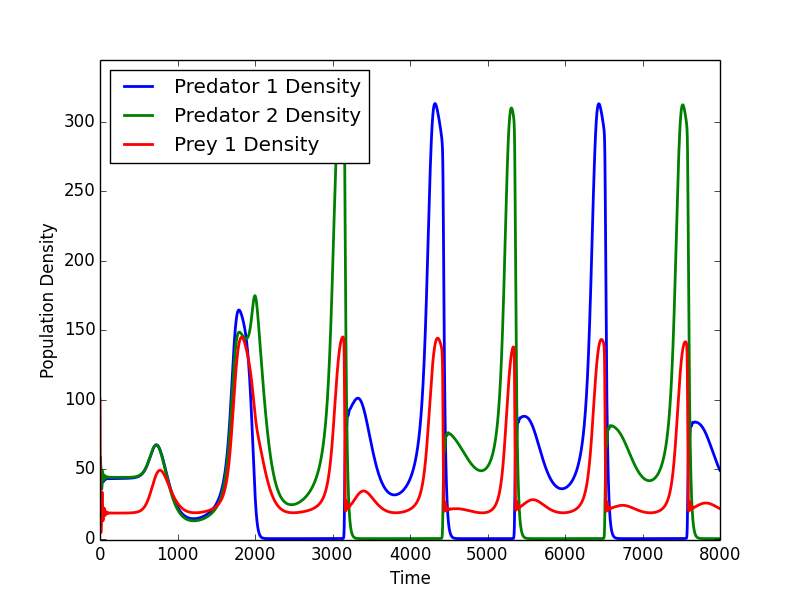
\includegraphics[width=5cm,height=3.75cm]{figures/2x1/variable_growth/densities_slow_prey_evo.png}\\
			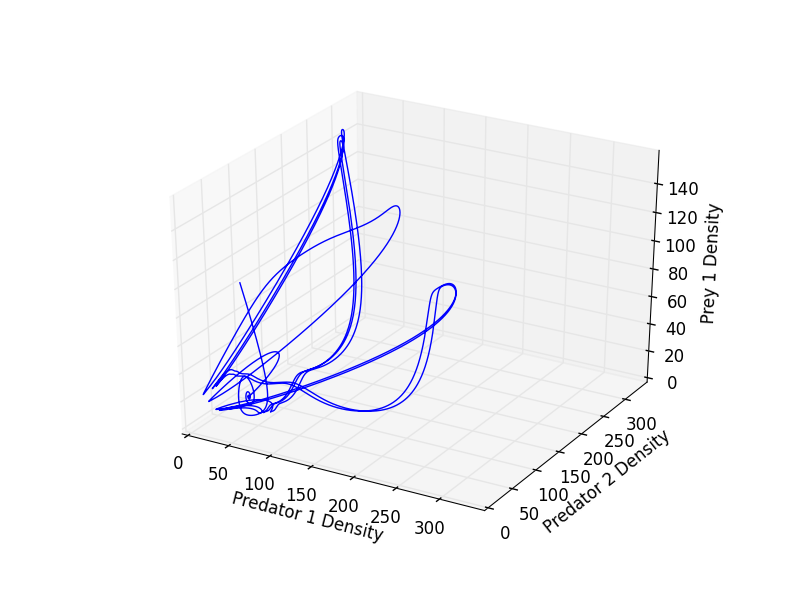
\includegraphics[width=5cm,height=3.75cm]{figures/2x1/variable_growth/density_phase_plane_slow_prey_evo.png}
		\end{column}
		\begin{column}{.5\textwidth}
			\centering
			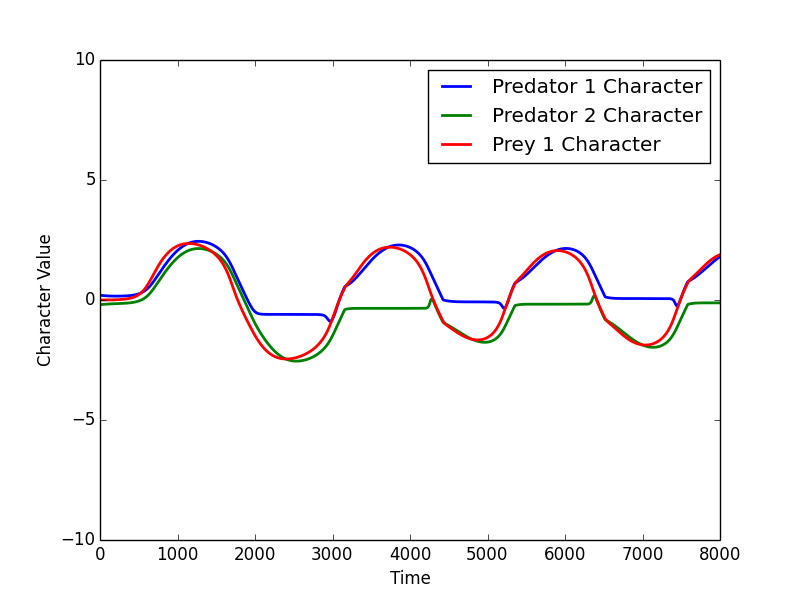
\includegraphics[width=5cm,height=3.75cm]{figures/2x1/variable_growth/traits_slow_prey_evo.png}\\
			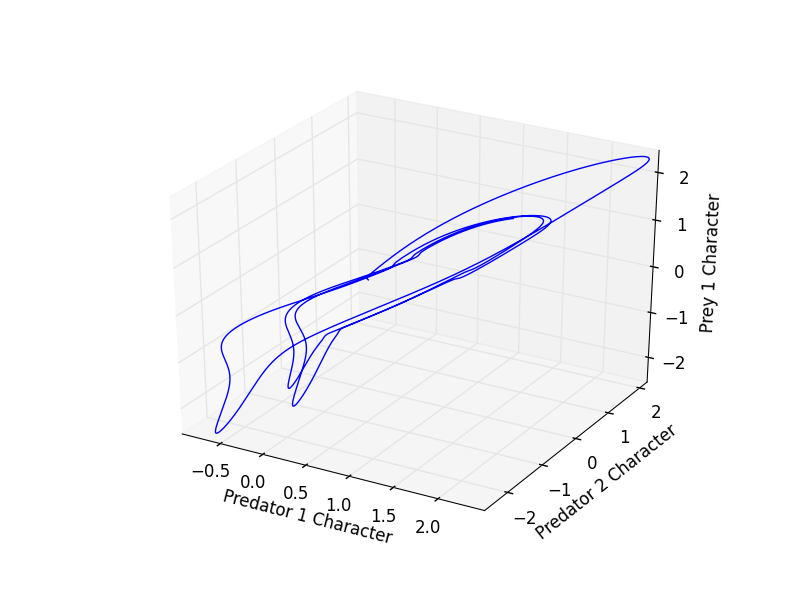
\includegraphics[width=5cm,height=3.75cm]{figures/2x1/variable_growth/trait_phase_plane_slow_prey_evo.png}
		\end{column}
	\end{columns}
\end{frame}
\begin{frame}
	\frametitle{Figures - $1\times2$}
	\begin{columns}[t]
		\begin{column}{.5\textwidth}
			\centering
			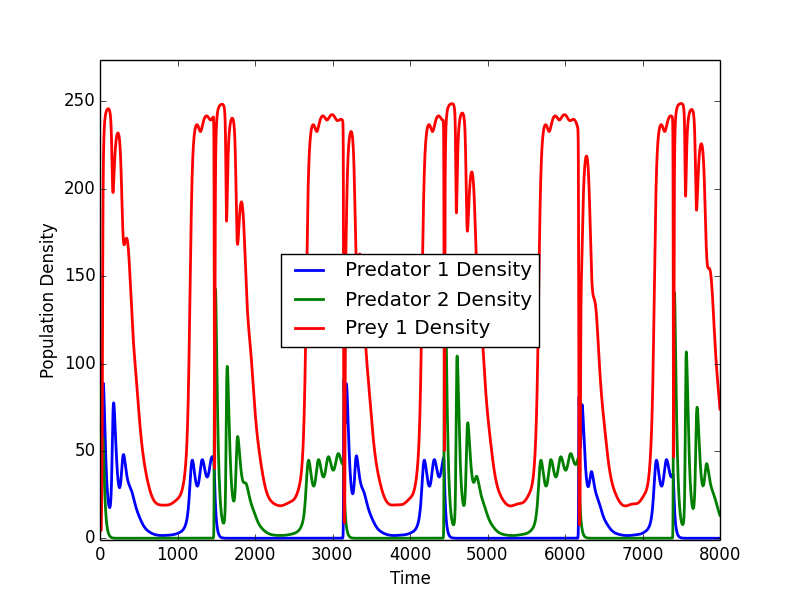
\includegraphics[width=5cm,height=3.75cm]{figures/2x1/variable_growth/densities_fast_prey_evo.png}\\
			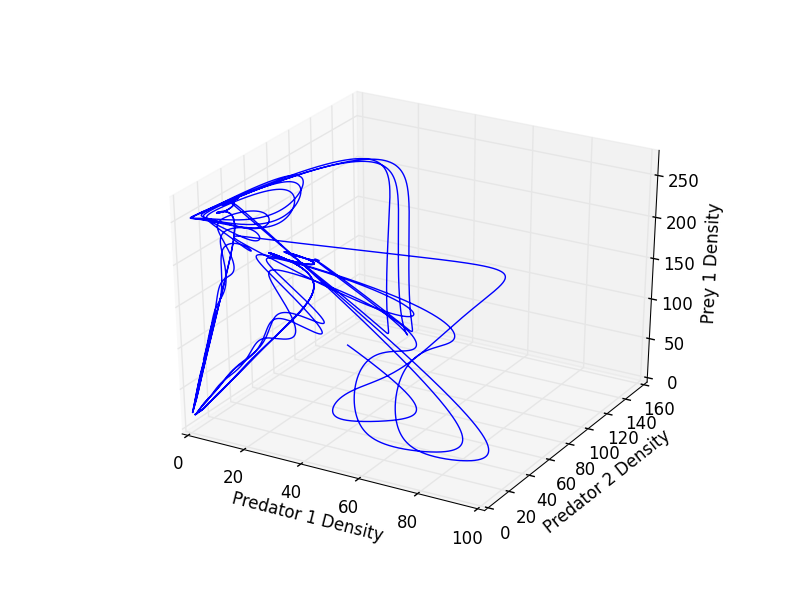
\includegraphics[width=5cm,height=3.75cm]{figures/2x1/variable_growth/density_phase_plane_fast_prey_evo.png}
		\end{column}
		\begin{column}{.5\textwidth}
			\centering
			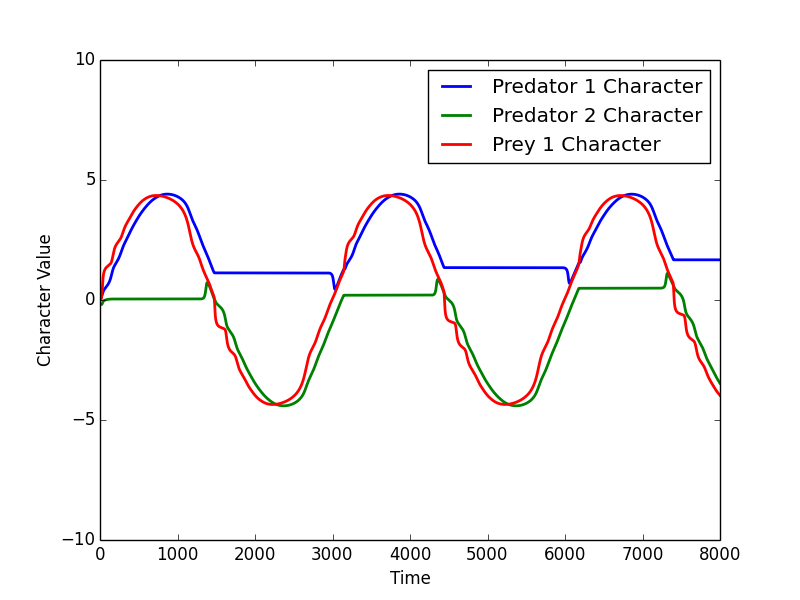
\includegraphics[width=5cm,height=3.75cm]{figures/2x1/variable_growth/traits_fast_prey_evo.png}\\
			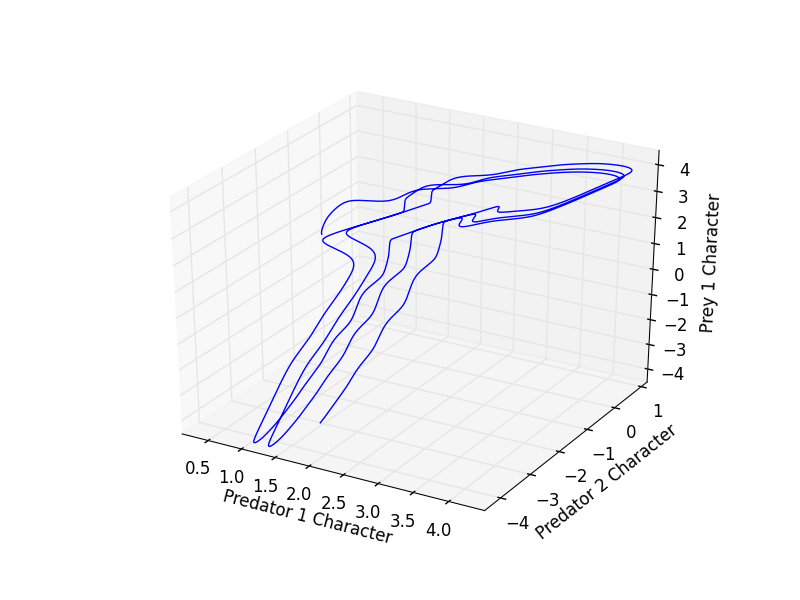
\includegraphics[width=5cm,height=3.75cm]{figures/2x1/variable_growth/trait_phase_plane_fast_prey_evo.png}
		\end{column}
	\end{columns}
\end{frame}

\subsection{Future Work}
\begin{frame}
	\frametitle{Future Work}
	\begin{itemize}
		\item \large ($1\times 2$) Two predator species in competition for one prey
		\item ($2\times 1$) Two prey species in apparent competition via one generalist predator
		\item ($2\times 2$) One specialist predator competing with one generalist predator for two prey
		\item ($2\times 3$) Two specialist predators competing with one generalist predator for two prey species
		\item ($u \times v$) The General Ditrophic Expansion
		\item Intraguild Predation and General Multitrophic Expansion
	\end{itemize}
\end{frame}

\begin{frame}
	\frametitle{Thank You!}
	\begin{itemize}
		\item PUMP (Preparing Undergraduates through Mentoring towards PhDs)
		\item The Pacific Math Alliance
		\item The National Math Alliance
		\item Dr. Helena Noronha, Dr. Ramin Vakilian, and all other PUMP organizers
		\item National Science Foundation
		\item California State University, Northridge
		\item Dr. Jing Li and Dr. Casey terHorst
	\end{itemize}
	\begin{center}
		{\Huge Questions?}
	\end{center}
\end{frame}

% \begin{frame}
% 	\frametitle{Equilibria - $1\times2$}
% 	\begin{align*}
% 		\begin{array}{ll}
% 			\dfrac{dN_1}{dt} = N_1\cdot \overline{Y}_1(\overline{m}, \overline{n}_1, M, N_1) &\ \ \ \ \ \ \dfrac{d\overline{n}_1}{dt} = \beta_{G1}^2\dfrac{\partial \overline{Y}_1}{\partial \overline{n}_1} \\[.3cm]
% 			\dfrac{dN_2}{dt} = N_2\cdot \overline{Y}_2(\overline{m}, \overline{n}_2, M, N_2) &\ \ \ \ \ \ \dfrac{d\overline{n}_2}{dt} = \beta_{G2}^2\dfrac{\partial \overline{Y}_2}{\partial \overline{n}_2} \\[.3cm]
% 			\dfrac{dM}{dt} = M\cdot \overline{W}(\overline{m}, \overline{n}_1, \overline{n}_2, N_1, N_2) & \ \ \ \ \ \ \dfrac{d\overline{m}}{dt} = \sigma_G^2\dfrac{\partial \overline{W}}{\partial \overline{m}}
% 		\end{array}
% 	\end{align*}
% 	\uncover<2->{{\bf Extinction}} \uncover<3->{$\boxed{\text{\it Unstable}}$}
% 	\begin{align*}
% 		\uncover<2->{(N_1^*, N_2^*, M^*, \overline{n}_1^*, \overline{n}_2^*, \overline{m}^*) = (0, 0, 0, \underline{\ \ }, \underline{\ \ }, \underline{\ \ })}
% 	\end{align*}
% 	\uncover<4->{{\bf Exclusion}} \uncover<5->{$\boxed{\text{\it Stable under certain conditions}}$}
% 	\begin{align*}
% 		\uncover<4->{(N_1^*, N_2^*, M^*, \overline{n}_1^*, \overline{n}_2^*, \overline{m}^*) &= (K_1, K_2, 0, \underline{\ \ }, \underline{\ \ }, \underline{\ \ })}
% 	\end{align*}
% \end{frame}
% \begin{frame}
% 	\frametitle{Equilibria - $1\times2$}
% 	\begin{align*}
% 		\begin{array}{ll}
% 			\dfrac{dN_1}{dt} = N_1\cdot \overline{Y}_1(\overline{m}, \overline{n}_1, M, N_1) &\ \ \ \ \ \ \dfrac{d\overline{n}_1}{dt} = \beta_{G1}^2\dfrac{\partial \overline{Y}_1}{\partial \overline{n}_1} \\[.3cm]
% 			\dfrac{dN_2}{dt} = N_2\cdot \overline{Y}_2(\overline{m}, \overline{n}_2, M, N_2) &\ \ \ \ \ \ \dfrac{d\overline{n}_2}{dt} = \beta_{G2}^2\dfrac{\partial \overline{Y}_2}{\partial \overline{n}_2} \\[.3cm]
% 			\dfrac{dM}{dt} = M\cdot \overline{W}(\overline{m}, \overline{n}_1, \overline{n}_2, N_1, N_2) & \ \ \ \ \ \ \dfrac{d\overline{m}}{dt} = \sigma_G^2\dfrac{\partial \overline{W}}{\partial \overline{m}}
% 		\end{array}
% 	\end{align*}
% 	\uncover<2->{{\bf Generalist Becomes Specialist}} \uncover<3->{$\boxed{\text{\it Stable under certain conditions???}}$}
% 	\begin{align*}
% 		\uncover<2->{&(N_1^*,N_2^*,M^*,\overline{n}_1^*,\overline{n}_2^*,\overline{m}^*) \\[.1cm]
% 		=\ &(\dfrac{d\sqrt{A_1}}{e_1 \alpha_1 \tau_1}\ ,\ K_2\ ,\ \dfrac{r_1\sqrt{A_1}}{\alpha_1\tau_1}\left(1 - \dfrac{d\sqrt{A_1}}{K_1e_1\alpha_1\tau_1}\right)\ ,\ \mu_1^*\ ,\ \mu_2^*\ ,\ \mu_1^* - \theta_1)}
% 	\end{align*}
% 	\uncover<2->{where $A_1 = \sigma^2 + \beta_1^2 + \tau_1^2$, $\mu_1^*$ is an arbitrary value, and $\mu_2^*$ is sufficiently far from $\mu_1^* - \theta_1$.}

% \end{frame}

% \begin{frame}
% 	\frametitle{Figures - $1\times2$}
% 	{\bf Generalist Becomes Specialist}
% 	\Wider[6em]{
% 	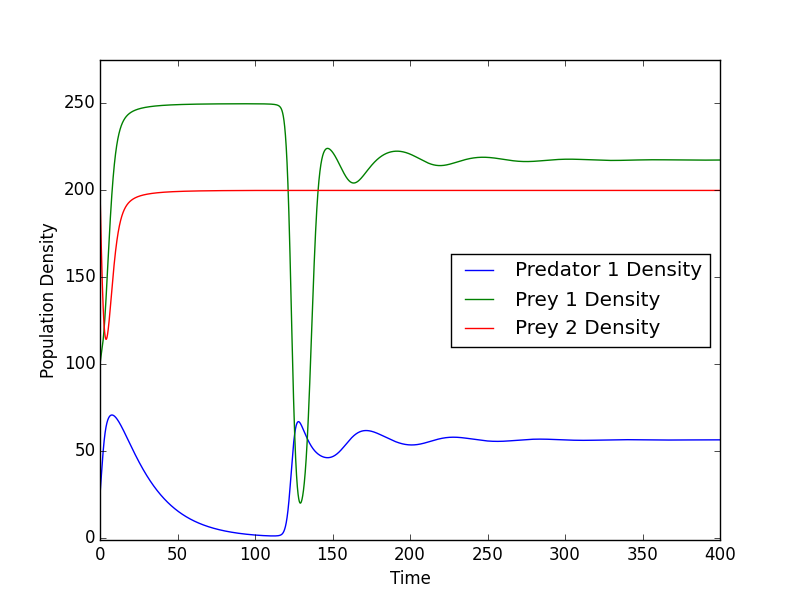
\includegraphics[scale=0.3175]{figures/1x2/densities_generalist_to_specialist.png}
%    	\hfill
%    	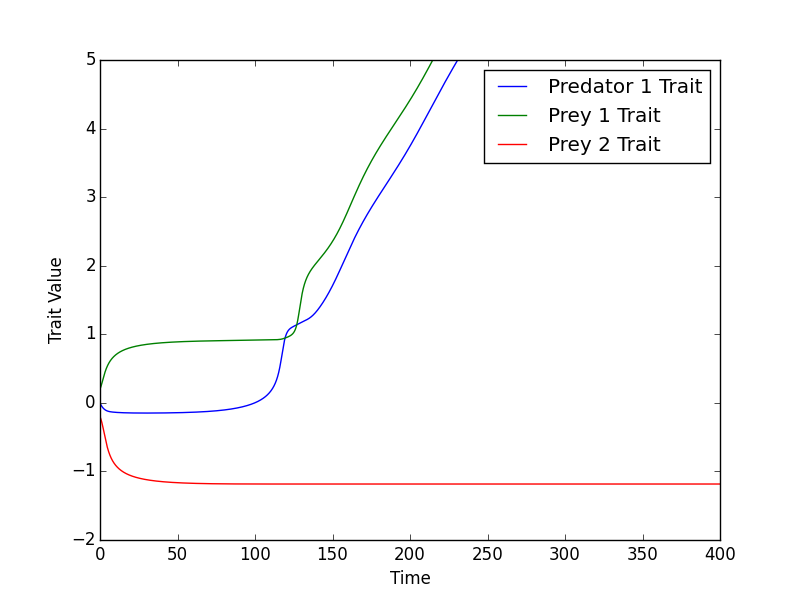
\includegraphics[scale=0.3175]{figures/1x2/traits_generalist_to_specialist.png}
% 	}
% \end{frame}
% \begin{frame}
% 	\frametitle{Figures - $1\times2$}
% 	{\bf Unstable Coexistence}
% 	\Wider[6em]{
% 	\includegraphics[scale=0.3175]{figures/1x2/densities_unstable_coexistence.png}
%    	\hfill
%    	\includegraphics[scale=0.3175]{figures/1x2/traits_unstable_coexistence.png}
% 	}
% \end{frame}





\end{document}